%% PRÄAMBEL

% -- Dokumentenklasse
\documentclass[
	% Schriftgröße
	11pt,
	% Papierformat
	a4paper,
	% Seitenverteilung
	oneside,
	% Sprache
	ngerman
	]{article}

% -- Schriftart Latin Modern verwenden (Vektor)
%\usepackage{lmodern}

% -- Schriftart Roboto Condensed verwenden (Vektor)
\usepackage[sfdefault]{roboto}

% -- Meta-Daten
\newcommand{\mytitle}{Pr\"aventive messtechnische Abbildung typischer Fertigungsabweichungen}
\newcommand{\myname}{Jan Doant}

% -- Seitenränder
\usepackage[left=30mm,right=20mm,top=25mm,bottom=20mm]{geometry}

% -- Zeilenabstand
\usepackage{setspace}
\makeatletter
\newcommand{\MSonehalfspacing}{%
	\setstretch{1.44}%  default
	\ifcase \@ptsize \relax % 10pt
	\setstretch {1.448}%
	\or % 11pt
	\setstretch {1.399}%
	\or % 12pt
	\setstretch {1.433}%
	\fi
}
\newcommand{\MSdoublespacing}{%
	\setstretch {1.92}%  default
	\ifcase \@ptsize \relax % 10pt
	\setstretch {1.936}%
	\or % 11pt
	\setstretch {1.866}%
	\or % 12pt
	\setstretch {1.902}%
	\fi
}
\makeatother
\MSonehalfspacing

% -- Deutsche Absatztrennung
\usepackage{parskip}

%% -- Gestaltung Kopf- und Fußzeile
% -- Kopfzeile
\usepackage{fancyhdr}
\addtolength{\headheight}{3pt}
\lhead{\mytitle}
% -- Fußzeile
\lfoot{\myname}
\cfoot{}
\rfoot{Seite~\thepage}  

%% -- deutsches Sprachpaket
% -- deutsche Silbentrennung
\usepackage[ngerman]{babel}
% -- Umlaute
\usepackage[utf8]{inputenc}
\usepackage[T1]{fontenc}
% -- deutsche Anführungszeichen
\usepackage[babel,german=quotes]{csquotes}

% -- Mathematikpakete
\usepackage{amsfonts}
\usepackage{amsmath}

% -- Grafikpaket
\usepackage{graphicx}

% -- Verweise 
% -- Verweise werden im Dokument klickbar
\usepackage[pdfpagelabels]{hyperref}
% -- Einfärben von Verweisen
\usepackage[dvipsnames,svgnames,x11names,hyperref]{xcolor}
\hypersetup{
	% Meta-Informationen, die in der PDF-Datei gespeichert werden
	pdfauthor={\myname},
	pdftitle={\mytitle},
	% Einfärben der Schrift
	colorlinks = true,
	% Farbe von Verknüpfungen im Text 
	linkcolor=[RGB]{63 81 181},
	% Farbe von Quellenverweisen
	citecolor= [RGB]{76 175 80},
	% Farbe von URLs
	urlcolor=[RGB]{0 76 153},
}

% -- Verweise automatisieren
%\usepackage{cleveref}
\usepackage{varioref}
\usepackage{prettyref}

% -- prettyref-Befehl konfigurieren
\newrefformat{fig}{Abbildung \vref{#1}}
\newrefformat{tab}{Tabelle \vref{#1}}

% -- Anzeigen der verwendeten Labels (nur im Dev-Modus verwenden)
\usepackage[
	% Label wird am inneren Rand angezeigt
	inner,
	% blendet Label aus, wenn final aktiv 			 
	final			 
	]{showlabels}

% -- Bibliografiestil
\usepackage[
	% Literaturverzeichnis wird in der Reihenfolge, in der die Referenzen genannt werden sortiert
	sorting=none,
	% keine Angabe der URL 		
	url=false,
	% Übersicht Biblatex-Styles:
	% https://de.sharelatex.com/learn/Biblatex_bibliography_styles 			
	style=ieee,
	% keine Angabe der ISBN 			
	isbn=false,
	% Datumsangabe nur für das Erscheiningsjahr
	date=year,
	% maximal 6 Namen in der Literaturliste
	maxbibnames=6,
	% mindestens 3 Namen in der Literaturliste    
	minbibnames=3,
	% Verwendung von biber.exe
	backend=biber
	]{biblatex}

% -- Pfad zur .bib-Datei
\addbibresource{bib/lit.bib}

% -- Tabellenpaket
\usepackage{tabularx}
\renewcommand{\arraystretch}{1.5}

% -- Verzeichnisse zum Inhaltsverzeichnis hinzufügen
\usepackage[
	% Inhaltsverzeichnis selbst nicht im Inhaltsverzeichnis aufführen 
	nottoc
	]{tocbibind}

% -- TikZ
\usepackage{tikz}

% -- Listings
\usepackage{listings}
\renewcommand{\lstlistingname}{Codebeispiel}
\lstdefinestyle{customc}{
	belowcaptionskip=1\baselineskip,
	breaklines=true,
	xleftmargin=2cm,
	language=[x86masm]Assembler,
	showstringspaces=false,
	basicstyle=\ttfamily,
	keywordstyle=\bfseries\color{green!40!black},
	commentstyle=\itshape\color{purple!40!black}
}

%% DOKUMENT
\begin{document}
	
% -- Titelseite
\pagenumbering{Alph}
\pagestyle{empty}
\begin{titlepage}
	
\begin{figure}[htbp]
	\begin{minipage}{0.19\textwidth}
		% \textwidth bezieht sich nun auf die Minipage
		
\includegraphics[width=\textwidth]{img/logo_tuc.pdf}
	\end{minipage}
	% Auffüllen des Zwischenraums
	\hfill
	% minipage mit Text
	\begin{minipage}{0.6\textwidth} 
		\begin{center}	
			Technische Universität Chemnitz\\
			Fakultät Maschinenbau\\
			Professur Fertigungsmesstechnik
		\end{center}
	\end{minipage}
	\hfill
	\begin{minipage}{0.19\textwidth} 
		% \textwidth bezieht sich nun auf die Minipage
		
\includegraphics[width=\textwidth]{img/logo_fmt.pdf}
	\end{minipage}
\end{figure}
	
	
	\vspace*{1cm}
		
		\begin{center}	
		
		\vspace{1.5cm}
		
		{\huge\textbf{Bachelorarbeit}}
		
		\vspace{1.5cm}
		
		{\large Arbeitstitel:}\\
		{\large\textbf{\mytitle}}
		
		\vspace{1.5cm}
		
		Betreuer: M.Sc. Robert Hofmann\\
		Prüfer: Univ.-Prof. Dr.-Ing. Sophie Gröger		
		
		\vfill
		
			
		
	\end{center}
	
	\begin{flushleft}
		Name: Jan Doant\\		
		E-Mail: jan.doant@s2017.tu-chemnitz.de\\
		Studiengang: Bachelor Maschinenbau (7. Semester)\\
		Matrikelnummer: 461311\linebreak
		
		
		Eingereicht am: 06.06.2018
		
	\end{flushleft}
	
	
\end{titlepage}
\newpage

% -- Inhaltsverzeichnis
\pagestyle{empty}
%%Anzahl der maximal aufgeführten Gliederungspunkte
\setcounter{tocdepth}{3}
\tableofcontents
\newpage

%% --Sandbox
%\pagestyle{fancy}
%\section{Sandbox}

\subsection{Sandbox--Zitierung}

Das ist zu eine zu zitierende Textstelle \cite{Klocke2008}.

\subsection{Sandbox--Längere Abschnitte}
Jemand musste Josef K. verleumdet haben, denn ohne dass er etwas Böses getan hätte, wurde er eines
Morgens verhaftet. Wie ein Hund! sagte er, es war, als sollte die Scham ihn überleben.

Als Gregor Samsa eines Morgens aus unruhigen Träumen erwachte, fand er sich in seinem Bett zu einem
ungeheueren Ungeziefer verwandelt. Und es war ihnen wie eine Bestätigung ihrer neuen Träume und
guten Absichten, als am Ziele ihrer Fahrt die Tochter als erste sich erhob und ihren jungen Körper
dehnte.
»Es ist ein eigentümlicher Apparat«, sagte der Offizier zu dem Forschungsreisenden und überblickte
mit einem gewissermaßen bewundernden Blick den ihm doch wohlbekannten Apparat. Sie hätten noch ins
Boot springen können, aber der Reisende hob ein schweres, geknotetes Tau vom Boden, drohte ihnen
damit und hielt sie dadurch von dem Sprunge ab.

In den letzten Jahrzehnten ist das Interesse an Hungerkünstlern sehr zurückgegangen. Aber sie
überwanden sich, umdrängten den Käfig und wollten sich gar nicht fortrühren. Jemand musste Josef K.
verleumdet haben, denn ohne dass er etwas Böses getan hätte, wurde er eines Morgens verhaftet. Wie
ein Hund! sagte er, es war, als sollte die Scham ihn überleben. Als Gregor Samsa eines Morgens aus
unruhigen Träumen erwachte, fand er sich



\subsection{Sandbox--Grafiken einbinden}

\begin{figure}[htbp] 
  \centering
     
\includegraphics[width=0.7\textwidth]{img/logo_tuc.pdf}
  \caption{Logo der Technischen Universität Chemnitz}
  \label{fig:Bild1}
\end{figure}

\newpage

\newpage


\subsection{Sandbox--Referenzierung}

Ich beziehe mich auf \prettyref{fig:Bild1}.
%\newpage

\pagenumbering{arabic}
\pagestyle{empty}
\addcontentsline{toc}{section}{Aufgabenstellung}
\section*{Aufgabenstellung}

Alle realen Fertigungsverfahren erzeugen gewisse charakteristische geometrische Abweichungen von der Nenngestalt, die zum Beispiel einem zeitlichen Trend oder einer zufälligen Auftretenswahrscheinlichkeit folgen. Ursache für diese Abweichungen sind dem jeweiligen Fertigungsverfahren innewohnende, teils unvermeidliche Erscheinungen. Zu diesen gehören zum Beispiel der Verschleiß des Werkzeugs oder äußere Schwingungen. 

Die beherrschte Vorhersage solcher Abweichungen ist bedeutend zur Absicherung der Produktqualität über die gesamte Produktionsstückzahl. Die Kenntnis über die sich wahrscheinlich einstellenden Ist-Abweichungen der Nenngestalt ist wichtig für verschiedene Prozesse der Fertigungsmesstechnik, wie zum Beispiel zur Definition der Messstrategie (Messpunktmuster, Messpunktanzahl, etc.). 

Ziel der Abschlussarbeit ist einerseits die umfassende Zusammenstellung und Kategorisierung charakteristischer geometrischer Fertigungsabweichungen. Darauf aufbauend ist ein geeignetes Werkzeug zu generieren, um die zu erwartenden Abweichungen durch eine erzeugte Punktewolke darzustellen.
Das geschieht, indem die vorhandene Soll-Geometrie durch einen geeigneten Algorithmus mit den erarbeiteten typischen Fertigungsfehlern beaufschlagt werden können. Dafür wird die Umsetzung mittels MATLAB oder einer geeigneten CAD-Software vorgeschlagen. 

\paragraph{Teilaufgaben}

\begin{itemize}
	\item Recherche und Katalogisierung von charakteristischen geometrischen Abweichungen, die aus realen Fertigungsverfahren hervorgehen können
	\item Erarbeitung eines Werkzeugs zur Erzeugung von erwartbaren Messpunktwolken durch die Beaufschlagung der Soll-Geometrie mit geometrischen Fertigungsabweichungen, zum Beispiel mittels MATLAB oder CAD
	\item Zusammenstellung der Erkenntnisse und Erarbeitung eines Ausblicks  
\end{itemize}
\newpage



% -- Einführung / Motivation
\pagestyle{fancy}
\section{Einführung}
\label{sec:einfuehrung}









\newpage

% -- Grundlagen / Stand der Technik
\pagestyle{fancy}
\section{Grundlagen}

\subsection{Oberflächenabweichungen und -unvollkommenheiten}

Um die Qualität einer technischen Oberfläche beurteilen zu können, ist es zunächst unerlässlich, verschiedene standardisierte Begriffe zu definieren. Dazu geben sowohl DIN 4760 als auch DIN EN ISO 8785 diverse Bezeichnungen vor, welche die möglichen auftretenden Oberflächenunvollkommenheiten voneinander abgrenzen und ordnen sollen.

\subsubsection{Wirkliche Oberfläche}

DIN 4760 definiert den Begriff der Wirklichen Oberfläche als die tatsächliche, den betrachteten Gegenstand von seinem Umgebungsmedium trennende Oberfläche. Für die Messtechnik ist diese Gestalt allerdings nicht in voller Gänze zu erfassen. Aus diesem Grund werden weitere Begriffe benötigt, um die Wirkliche Oberfläche zu abstrahieren und für die Messtechnik verfügbar zu machen. 

\subsubsection{Istoberfläche}

Als Istoberfläche bezeichnet die oben beschriebene Norm das messtechnisch erfasste Abbild der Wirklichen Oberfläche eines Formelementes. Dabei ist festzuhalten, dass hier von einer bereits vereinfachten Oberfläche zu sprechen ist. Abhängig von Messverfahren, Messparametern, Messplan und Messabfolge ergeben sich für verschiedene Messungen auch unterschiedliche Istoberflächen des Objektes. Dies ist bei der Betrachtung und Analyse einer Istoberfläche stets zu beachten. Natürlich wirken sich auch systematische und zufällige Messfehler auf die Gestalt der Istoberfläche aus. Um von der messtechnisch erfassten Gestalt des Bauteils auf dessen Gestaltabweichungen schließen zu können, ist der nachfolgende Begriff der Geometrischen Oberfläche unerlässlich. 

\subsubsection{Geometrische Oberfläche}

Als Geometrische Oberfläche wird in DIN 4760 die ideale Form des betrachteten Objektes definiert. Sie wird auch als Nennform bezeichnet und ist durch die jeweiligen technischen Zeichnungen oder andere technische Unterlagen, wie zum Beispiel 3D-CAD-Informationen festgeschrieben. Da kein Fertigungsprozess fehlerfrei abläuft, ist es unmöglich, diese Idealgeometrie in der Realität zu fertigen. Allerdings ist es mit Hilfe der technischen Dokumente möglich, zulässige Abweichungen von der Idealgeometrie festzulegen. Vielmehr dient diese Beschreibung in der Messtechnik als Referenz, um die im folgenden Abschnitt behandelten Gestaltabweichungen überhaupt erst erfassbar zu machen.
     
\subsubsection{Gestaltabweichungen}

Als Gestaltabweichungen werden in der beschreibenden Norm die Gesamtheit aller Abweichungen der messtechnisch erfassten Istoberfläche von der idealen geometrischen Oberfläche bezeichnet. Grundlage für das Vorhandensein von Gestaltabweichungen sind mannigfaltig und werden in den folgenden Abschnitten weiter ausgeführt. Grundsätzlich ist festzustellen, dass unterschieden wird zwischen solchen Abweichungen, die nur durch Betrachtung des gesamten Objektes feststellbar sind, und Abweichungen, die nur durch Analyse eines Ausschnittes der Oberfläche erkennbar werden (siehe Abb.\ref{fig:din4760_1}). Dazu werden die Gestaltabweichungen in 6 verschiedenen Ordnungen klassifiziert. 


\begin{figure}[h]
	\centering
	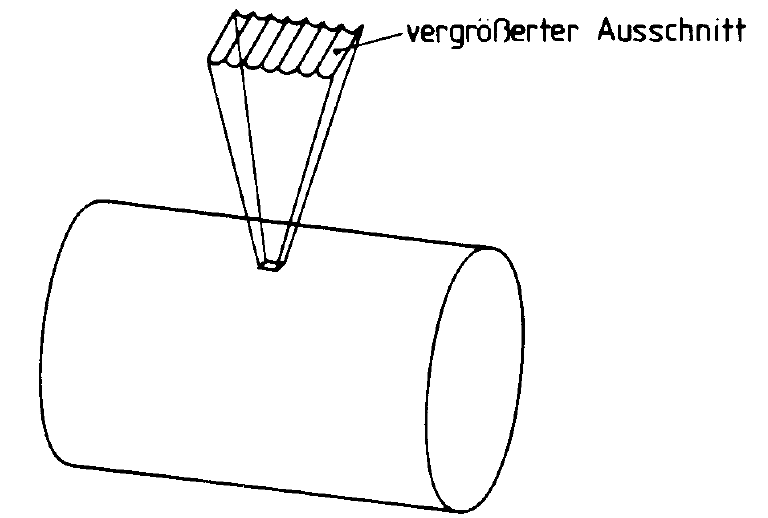
\includegraphics[width=0.5\linewidth]{img/DIN_4760_1}
	\caption[Ausschnitt aus der Istoberfläche zur Beurteilung der Gestaltabweichung]{Ausschnitt aus der Istoberfläche}
	\label{fig:din4760_1}
\end{figure}

Als Gestaltabweichungen 1. Ordnung werden in DIN 4760 jene Gestaltabweichungen beschrieben, die, wie weiter oben bereits angeschnitten, bei der Beurteilung der gesamten Istoberfläche ersichtlich werden. Abweichungen dieser Kategorie werden als Formabweichungen bezeichnet. Darunter zählen beispielsweise Geradheits-, Ebenheits- und Rundheitsabweichungen. Diese Art der Abweichungen begründet die Norm in fehlerhaften Führungen der bearbeitenden Maschine, Durchbiegung von Werkzeug oder Werkzeugmaschine, falscher Einspannung des Werkstückes, Verschleiß oder Härteverzug.

Die 2. Ordnung der Gestaltabweichungen wird unter dem Begriff Welligkeit geführt. Es handelt sich dabei um periodisch wiederholt auftretende Gestaltabweichungen der gemessenen Oberfläche eines untersuchten Formelements. Als wellig definiert die Norm DIN 4760 Abweichungen, bei denen das Verhältnis von Wellenabständen zur Wellentiefe generell zwischen 1000 : 1 und 100 : 1 liegt. Es handelt sich also um relativ niederfrequente Wellen mit einer verhältnismäßig niedrigen Amplitude. Als grundlegende Ursachen für die Entstehung von welligen Formen nennt die Norm sowohl außermittige Einspannung des Werkstücks als auch Form- und Laufabweichungen des Werkzeugs und Schwingungen der Werkzeugmaschine und des Werkzeugs.

Die Gestaltabweichungen 3. bis 5. Ordnung werden als Rauheit bezeichnet. Sie sind nur durch Betrachtung eines Oberflächenausschnitts des Objektes zu erkennen. Rauheitsabweichungen kehren entweder regelmäßig oder unregelmäßig wieder. Sie sind gekennzeichnet durch ein Verhältnis der Abstände zur Tiefe zwischen 100 : 1 und 5 : 1. Es handelt sich also im Vergleich zum im vorherigen Abschnitt beschriebenen Welligkeitsphänomen um hochfrequentere Abweichungen der Oberfläche. 
Innerhalb der Klasse der Rauheitsabweichungen lassen sich verschiedene Ausprägungen beschreiben. So unterscheidet die Norm Rillen (4. Ordnung), Riefen, Schuppen, Kuppen (5. Ordnung) und Oberflächenrauheit, welche durch die Gefügestruktur hervorgerufen wird (6. Ordnung).
Diese Kategorien unterscheiden sich in Frequenz und Amplitude ihrer Form (siehe Abb. *Todo*). Außerdem lassen sich verschiedene Ursachen für ihr Auftreten finden. 

Rillen werden durch die Form der Werkzeugschneide sowie aufgrund des eingestellten Vorschubes und der Schnittbewegung des Werkzeuges hervorgerufen.
Riefen, Schuppen und Kuppen sind Oberflächenunvollkommenheiten, deren Gründe im Prozess der Spanbildung zu finden sind. Des Weiteren lassen sie sich beispielsweise durch Werkstoffverformung beim Strahlen oder Knospenbildung bei galvanischer Behandlung erklären. 

Rauheiten, welche durch die Gefügestruktur des Werkstoffes verursacht werden, sind durch Kristallisationsvorgänge oder Veränderungen der Oberfläche beispielsweise durch chemische oder korrosive Vorgänge entstanden. Sie bilden zusammen mit der 6. Ordnung der Gestaltabweichungen, welche durch den Gitteraufbau des Materials zu erklären sind, die nicht mehr durch Messverfahren ermittelbaren Gestaltabweichungen. 

Das bedeutet, dass in der Istoberfläche für gewöhnlich eine Struktur zu erkennen ist, die durch Überlagerung der Gestaltabweichungen 1. bis 4. Ordnung verursacht wird. 

\subsubsection{Oberflächenunvollkommenheiten}

Zusätzlich zu den in DIN 4760 aufgeführten Gestaltabweichungen werden in DIN EN ISO 8785 Oberflächenunvollkommenheiten erläutert. In der Norm werden diese als "`Element, Unregelmäßigkeit oder Gruppe von Elementen und Unregelmäßigkeiten der Wirklichen Oberfläche, die unbeabsichtigt oder zufällig durch die Bearbeitung, Lagerung oder Funktion der Oberfläche entstanden sind"' definiert. Es wird dabei unterschieden zwischen nach innen orientierten (Vertiefung), nach außen gerichteten (Buckel), kombinierten und stellenweisen Oberflächenunvollkommenheiten. Kombinierte Oberflächenunvollkommenheiten enthalten sowohl Anteile von Vertiefungen als auch Buckeln. Stellenweise Unvollkommenheiten besitzen eine kaum messbare Erhöhung bzw. Vertiefung. 

In \prettyref{fig:din-en-8785-beispiele} sind einige Beispiele für jede genannte Kategorie der Oberflächenunvollkommenheiten zu finden. 

\begin{figure}[h]
	\centering
	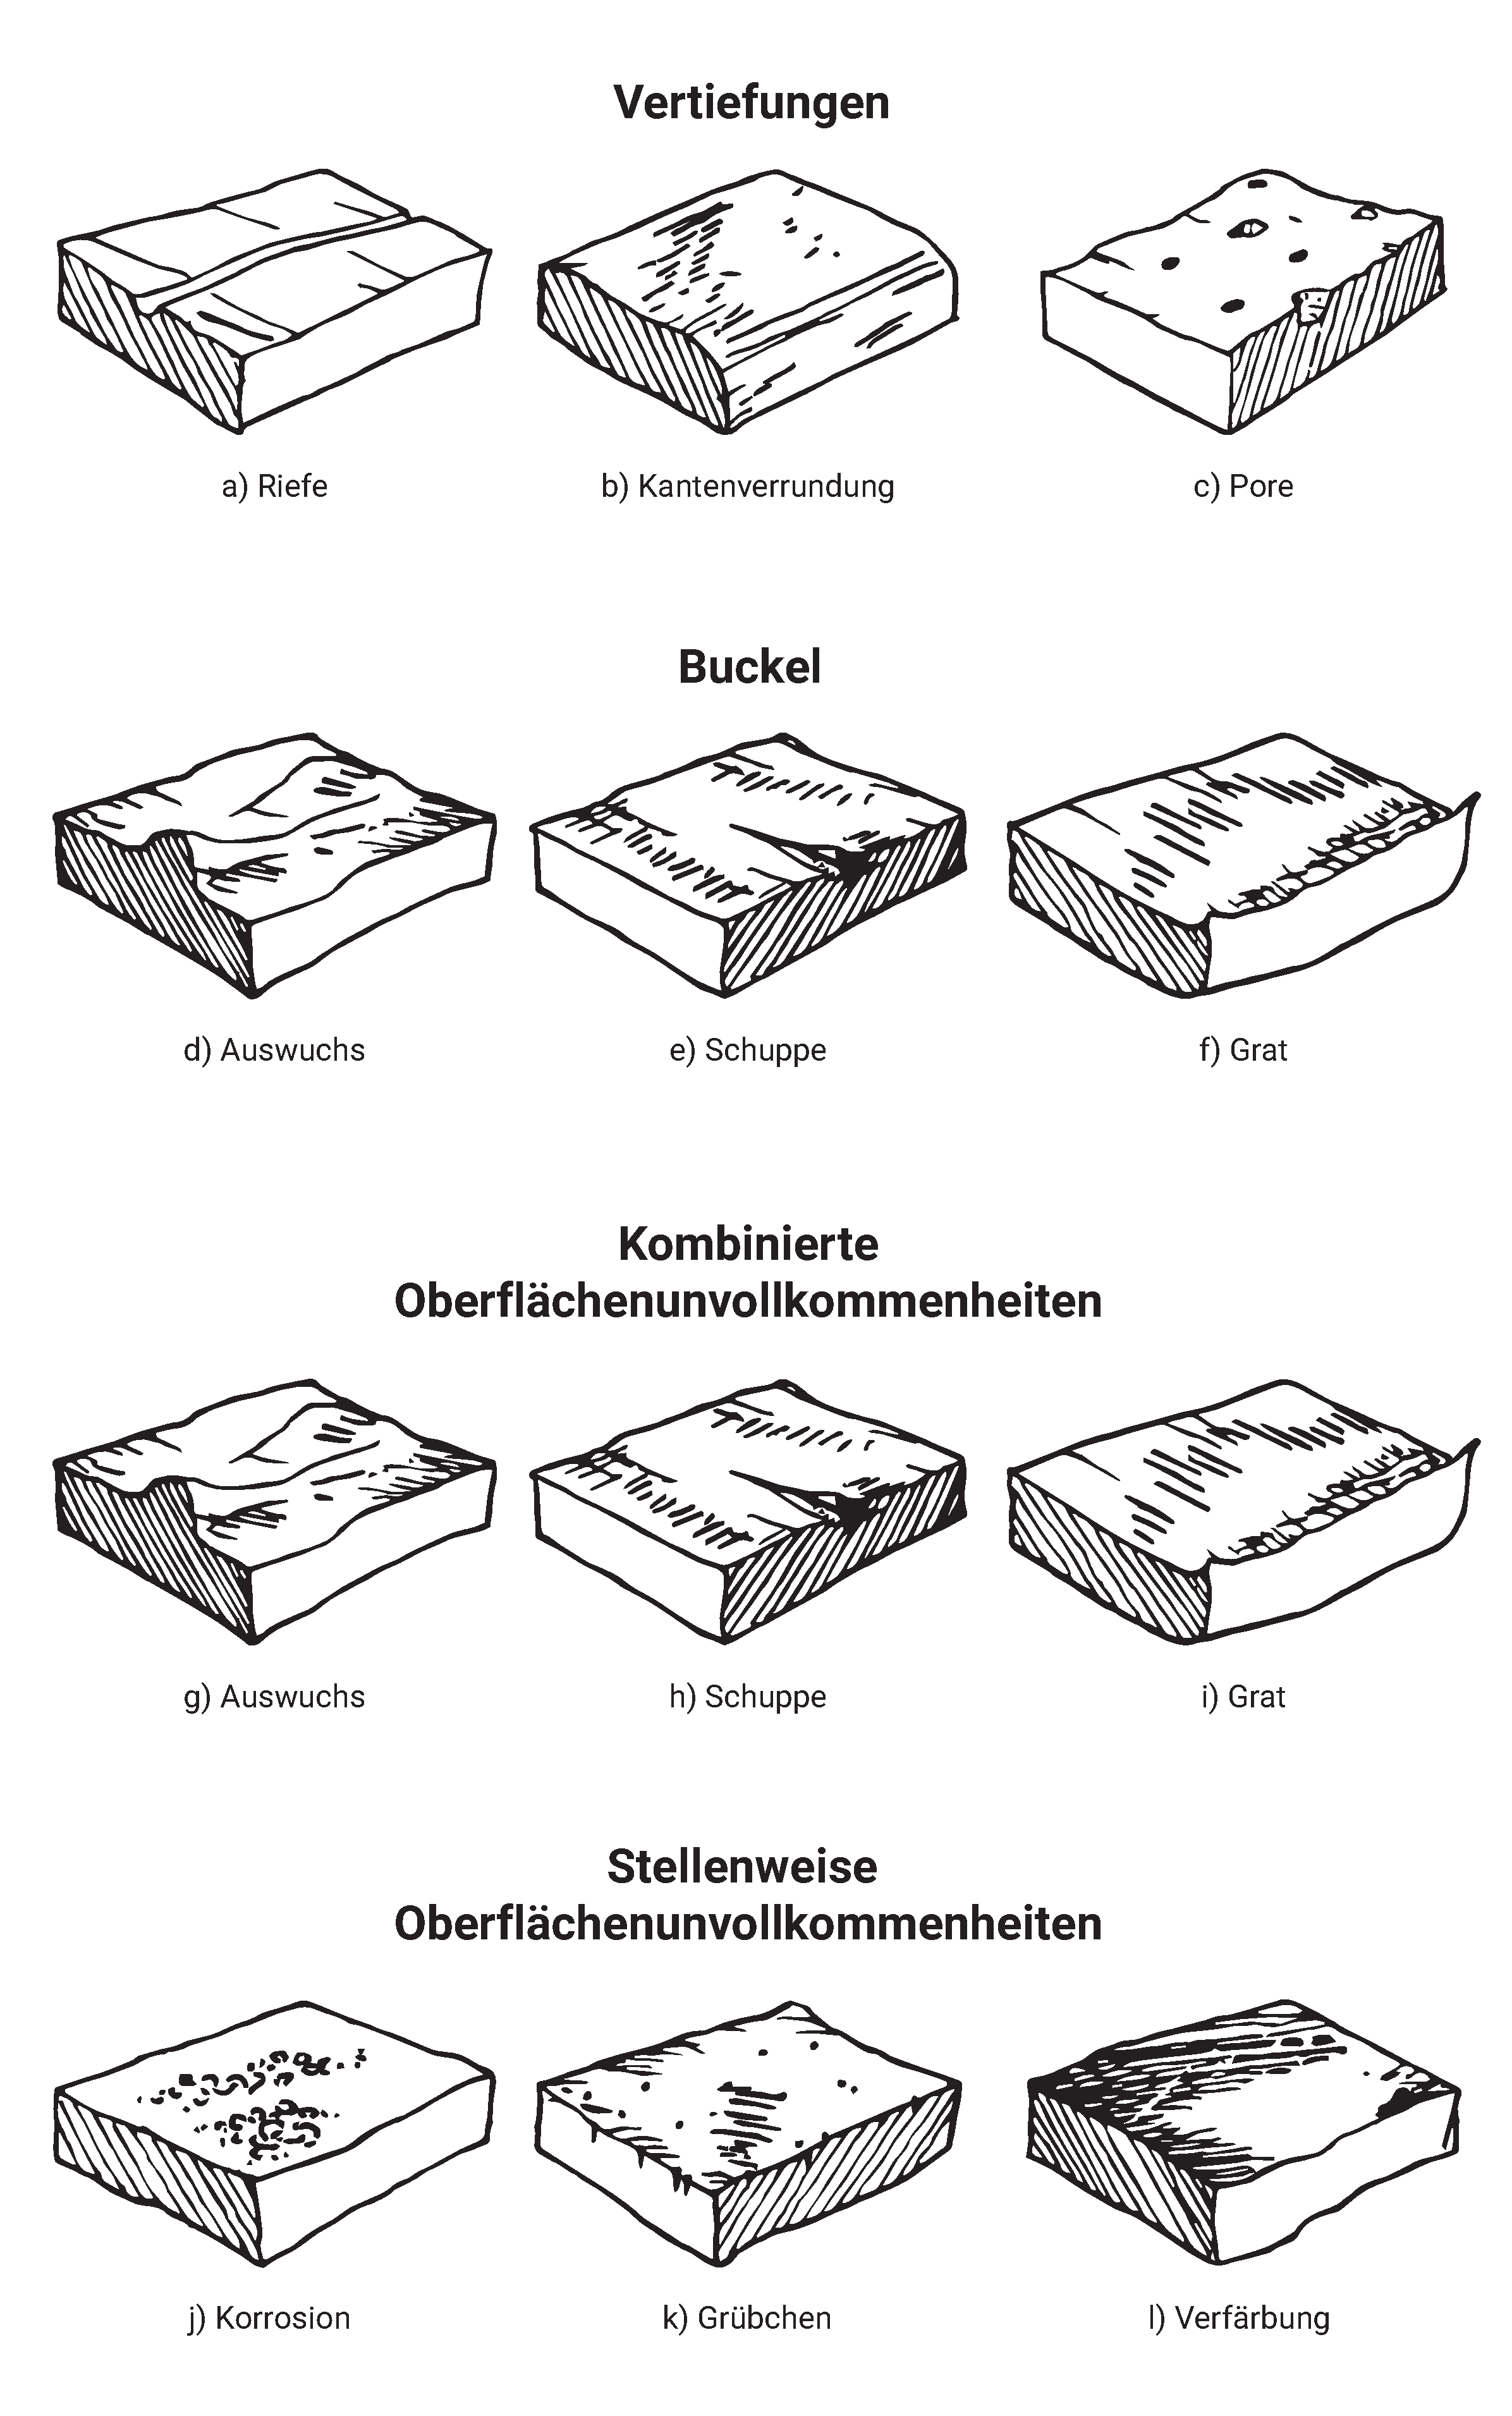
\includegraphics[width=0.7\linewidth]{img/din_en_8785_beispiele}
	\caption[DIN EN ISO 8785 - Oberflächenunvollkommenheiten]{DIN EN 8785 - Oberflächenunvollkommenheiten}
	\label{fig:din-en-8785-beispiele}
\end{figure}









 






          




\subsection{Typische Abweichungen bei verschiedenen spanenden Fertigungsvefahren}

\subsubsection{Ursachen für Fertigungsabweichungen}

Jedes Bauteil, welches in einem Fertigungsverfahren hergestellt wird, entspricht in seiner Realgestalt nicht der in den Fertigungsunterlagen (Technische Zeichnung oder CAD-Modell) festgehaltenen Idealgeometrie. Es sind durch verschiedene Einflüsse stets Abweichungen von der Geometrischen Oberfläche des Objektes festzustellen. Dies hat nach \cite{Denkena.2011} verschiedene Ursachen, die im Werkstück selbst, dem bearbeitenden Werkzeug, der Werkzeugmaschine oder der Fertigungsumgebung liegen. 

So werden als Ursachen für Fertigungsabweichungen, die durch das Werkzeug bestimmt werden, bereits vorhandene Form- und Lagetoleranzen des Rohteils, Festigkeitsunterschiede der abzuspanenden Teile, Auslösung bzw. Einbringung von Eigenspannungen in das Werkstück und örtlich und zeitlich veränderliche Temperaturfelder im Bauteil genannt.
Es ist festzuhalten, dass Wärmeeinbringung am Werkstück vor allem Formfehler zur Folge hat. Bei zylindrischen Bauteilen zeigen sich diese hauptsächlich in axialer Richtung wegen inhomogener elastischer Erwärmung.

Weiterhin hat auch das bearbeitende Werkzeug einen sehr großen Einfluss auf die Wirkliche Geometrie des Bauteils. Hier sind besonders die Nachgiebigkeit des Werkzeugs bzw. Werkzeughalters, die Lageabweichung des Werkzeugs beim Werkzeugwechsel sowie der Verschleiß des Werkzeugs zu nennen. Dabei hat der Werkzeugverschleiß einen maßgeblichen Einfluss auf die Maß- und Formgenauigkeit. Werkzeugverschleiß führt zu Schneidenversatz, dies wiederum begründet die Fehler, die die Maßhaltigkeit betreffen. Die Formabweichungen sind in den durch den Werkzeugverschleiß auftretenden höheren Schneidkräften bedingt. Diese führen zusammen mit der Nachgiebigkeit der Werkzeugmaschine zum Auftreten dieser Abweichungen.

Der Einfluss der bearbeitenden Maschine liegt in ihrer Nachgiebigkeit im Kraftfluss und ihrer thermischen Wirkung. So kommt es zu geometrischen Abweichungen und thermisch bedingten Verformungen während des Bearbeitungsprozesses. Ungenauigkeiten in den Führungen der Werkzeugmaschine führen über die kinematische Kette der Maschine zu sich fortpflanzenden geometrischen Fehlern im Bauteil \cite{Neugebauer.2012}.

Auch die Umgebung der Maschine wirkt natürlich auf die Werkstückqualität ein. So führen externe Wärmequellen, Änderungen der Umgebungstemperatur oder eine Veränderung der Kühlschmierung zu Abweichungen am Werkstück. Zählt man den Bearbeiter des Bauteils zu den Umgebungsfaktoren hinzu, ergeben sich auch durch systematische oder zufällige menschliche Fehler in der Einrichtung und Überwachung des Bearbeitungsprozesses Einflüsse auf die Formgestalt des Bauteils. 

Es ist festzuhalten, dass ein komplexes System an Einflussfaktoren auf das Werkstück einwirkt, die sich gegenseitig beeinflussen können. Es ist nicht möglich, ohne detaillierte Kenntnis aller Faktoren bereits im Vorfeld konkret vorherzusagen, welche Abweichungen bei einem Fertigungsverfahren zu erwarten sind. Durch Erfahrungswerte lassen sich allerdings typische Abweichungen für die einzelnen Fertigungsverfahren beschreiben. 

\subsubsection {Fertigungsabweichungen beim Drehen}

Beim Fertigungsverfahren Drehen sind, je nach konkretem Drehverfahren, unterschiedliche Maßtoleranzen zu erreichen. So sind laut \cite{Dietrich.2014} beim Schlichtdrehen Toleranzen von IT7 bis IT8 realistisch, beim Feinschlichten können unter optimalen Drehbedingungen sogar Genauigkeiten von IT6 umgesetzt werden. Das deckt sich mit den Angaben nach \cite{Denkena.2011}, wonach mit konventionellen Drehmaschinen Maßabweichungen von IT6 bis IT7 realisierbar sind. Ergänzend dazu werden mögliche Rundheitsabweichungen auf konventionellen Drehmaschinen von weniger als 2,5 µm, Zylindrizitätsabweichungen von weniger als 2 µm und gemittelte Rautiefen $R_{z}$ von 2 bis 6 µm beschrieben. 

Außerdem wird die mögliche Fertigungsgenauigkeit von Präzisionsdrehmaschinen genannt. Dabei werden Maßabweichungen im Bereich von IT5 bis IT6, Rundheitsabweichungen von 0,2 µm, Zylindrizitätsabweichungen von weniger als 0,1 µm sowie eine gemittelte Rautiefe $R_{z}$ von 0,5 µm erreicht. Dies ist also ein deutlich genaueres Verfahren, was bei der Betrachtung der zu erwartenden Abweichungen unbedingt in Erwägung gezogen werden muss. 

Die theoretische Oberflächenrauheit einer drehend hergestellten Oberfläche lässt sich laut \cite{Dietrich.2014} und \cite{Paucksch.2008} mit der Formel 

\begin{equation*}
	R_{t}=\frac{f^{2}}{r_{\epsilon}}
\end{equation*}

berechnen. In dieser Formel beschreibt $r_{\epsilon}$ den Eckenradius und $f$ den Vorschub des Werkzeugs in axialer Richtung. Die Vorschubgeschwindigkeit hat demnach einen quadratischen Einfluss auf die theoretische Oberflächenrauheit und gibt diese maßgeblich vor. Mit zunehmender Nutzungsdauer des Werkzeuges steigt dessen Verschleiß, wobei sich somit der Betrag des Eckenradius stets ändert. Dies resultiert laut oben genannter Formel aus einer Veränderung der Oberflächengüte des bearbeiteten Geometrieelements. 

Drehende Verfahren weisen eine stark gerichtete Bearbeitungsrichtung auf, weshalb durchweg gerichtete, rillige Oberflächen entstehen. Diese gerichteten Oberflächen weisen in der Regel quer zur Schnittrichtung größere Rauheiten als in Schnittrichtung auf \cite{Denkena.2011}.
Diese Rillen sind stark geprägt von der Form und dem Verschleißzustand des Drehmeißels sowie der Vorschubbewegung \cite{Paucksch.2008}.
Weiterhin ist die Oberflächenrauheit geprägt von der Zerspanbarkeit des Werkstoffes. Eine gute Zerspanbarkeit ermöglicht geringe Fehler in der Form und Oberflächengüte des Bauteils. Werkstoffe mit einer homogenen Gefügeausbildung erreichen eine höhere Arbeitsgüte einfacher als Werkstücke mit Fehlstellen (z. B. Lunker oder Porositäten).

Wie alle Verfahren erzeugt auch das Drehen erfahrungsgemäß typische Fehler am Werkstück, die konkreten Ursachen zugeordnet werden können. Dies ermöglicht den Rückschluss vom Fehlerbild auf die Ursache und erlaubt eine Anpassung der Prozessparameter, um eine höhere Arbeitsgenauigkeit zu steuern. 

Ungenügende Maßgenauigkeit lässt sich zum Beispiel über einen zu hohen Verschleiß des Werkzeuges erklären. Mit übermäßigem Verschleiß wird der Schneidkantenversatz des Drehmeißels zu groß, was eine kontrollierte Einstellung der Oberflächenrauheit erschwert. Eine weitere Ursache für zu hohe Maßabweichungen kann in einer Durchbiegung des eingespannten Werkstückes liegen. Dies resultiert aus zu hohen Passivkräften bei der Zerspanung (zu hohe Schnitttiefe oder Werkzeugvorschub), fehlender Abstützung schlanker Werkstücke oder einem zu hohen Einstellwinkel $\kappa$ des Werkzeuges \cite{Schonherr.2002}.

Ein weiterer Fehler, der sich bei drehend hergestellten Bauteilen finden lässt, ist die Unrundheit des Profils außerhalb der vorgegebenen Toleranzen. Ein Grund dafür liegt in der übermäßigen Durchbiegung des Bauteils aus den oben genannten Gründen. Außerdem wirken sich eine ungenaue, außermittige Zentrierung, Längsführungen oder Hauptspindellagerungen mit zu viel Spiel und elastische Verformungen des Werkstückes durch zu hohe Spannkräfte negativ auf die Rundheit des Bauteils aus \cite{Dietrich.2014}, \cite{Schonherr.2002}. 

Bei Drehteilen lassen sich außerdem wellige Oberflächen feststellen. Dies ergibt sich aus Schwingungen der Drehmaschine und damit auch des Werkzeugs im Eingriff durch zu hohes Spiel in den Führungen der Maschine. Außerdem führen eine falsche Werkzeugeinspannung und zu hohe Schnittleistungen zum Einbringen von zusätzlichen Schwingungen in die Werkzeugmaschine, was die Bildung welliger Oberflächen begünstigt \cite{Dietrich.2014}. 

Rattermarken am Werkstück entstehen aufgrund eines instabilen Werkzeugs (Auskraglänge zu groß, Schaftquerschnitt zu gering oder instabile Einspannung), zu hohen Passivkräften bei der Bearbeitung, einem zu hohen Freiflächenverschleiß oder einer ungenügenden Schneidkantenschärfe des Werkzeugs, beispielsweise wegen einer Beschichtung dessen \cite{Schonherr.2002}.

Eine konische Form des angestrebten zylindrischen Bauteils entsteht laut \cite{Dietrich.2014} aufgrund einer nicht fluchtenden Anordnung von Drehachse der Maschine und Achse der Reitstockspitze. 

Kratzer auf der Oberfläche eines Drehteils lassen sich auf Oxidationsverschleiß der Nebenschneide des Werkzeugs oder auf den Kontakt mit Spänen zurückführen, welche die fertig gedrehte Oberfläche beschädigen \cite{Schonherr.2002}. 

\subsubsection {Fertigungsabweichungen beim Bohren}

Beim Fertigungsverfahren Bohren sind verschiedene Maßtoleranzen und Rautiefen zu erreichen. Auch beim Bohren sind die Werte stark von dem Bohrverfahren und den Prozessparametern abhängig.
\prettyref{tab:bohrungsqualitaet} stellt den Sachverhalt anschaulich dar:

\begin{table}[h]	
	
	\begin{tabularx}{\columnwidth}{|X|c|c|l|}	
		\hline
		\textbf{Verfahren}&\textbf{Maßtoleranz}&\textbf{Rautiefe $R_{t}$ in µm}&\textbf{Oberflächenqualität}\\
		\hline
		Bohren ins Volle&IT12&80&Schruppen\\
		\hline
		Aufbohren mit Wendelsenkern&IT11&20&Schlichten\\
		\hline
		Senken mit Flach- und Form\-senkern&IT9&12&Schlichten\\
		\hline
		Reiben&IT7&8&Feinschlichten\\
		\hline
		Ausdrehen mit Ausdrehmeißel oder mehrschneidigem Bohrkopf&IT7&8&Feinschlichten\\
		\hline
		Ausdrehen mit Hartmetallschneiden und sehr kleinem Spanungsquerschnitt&IT7&4&Feinschlichten\\
		\hline
		
	\end{tabularx}
	
	\caption{Maßtoleranzen und Rautiefen verschiedener Bohrverfahren (Quelle: \cite{Dietrich.2014})}
	\label{tab:bohrungsqualitaet}

\end{table}

Des Weiteren beschreibt \cite{Schonherr.2002} die Abhängigkeit der erreichbaren Genauigkeiten vom Material des Bohrers. So sind mit HSS-Spiralbohrern Toleranzen von IT12, mit Vollhartmetall-Spiralbohrern Toleranzen von IT9 und mit geradgenutetem Vollhartmetallbohrer Toleranzen von IT7 herstellbar. 

Generell ist zu sagen, dass ein Bohren ins Volle mit einem Wendelbohrer stets eine Schruppbearbeitung darstellt. Das heißt, es ist keine hochgenaue Fertigung möglich. Viel bessere Genauigkeiten lassen sich mit Reiben, Senken, Feinbohren und Ausdrehen erzielen \cite{Schonherr.2002}.

Die Formgenauigkeit einer Bohrung wird hauptsächlich durch deren Rundheit und Geradheit beschrieben. Mangelnde Formgenauigkeit kann verschiedene Ursachen haben. Dazu zählen eine nicht ausreichend hohe Steifigkeit von Werkzeugmaschine, Werkzeug und der Werkzeugaufnahme. Weiterhin wirken sich eine schlechte Zentrierung beim Anschnitt, ungleichmäßiges Schneiden aller Hauptschneiden des Bohrers und zu hohe Belastungen (Vorschub- und Schnittkräfte) negativ auf die Formhaltigkeit der Bohrung aus. Positiv können sich hingegen die Verwendung geradgenuteter oder rechtsgedrallter Bohrer und eine gute Spanbildung (Spanformung, Spanbruch, Spanabfuhr) niederschlagen. 

Von Werkzeugen verursachte Asymmetrien unterscheiden sich deutlich von werkstückbedingten Asymmetrien. Dadurch entstehen typische Bohrfehler.

Durch ungünstige Werkzeuge zu begründende Fehler bohrend hergestellter Flächen sind beispielsweise Überweite und Konizität des Geometrieelements. Dabei sind nach [Paucksch] vor allem durch Anschlifffehler erzeugte asymmetrische Werkzeuge ursächlich. Diese sind charakterisiert durch Hauptschneidenlängenunterschiede, Einstellwinkeldifferenzen, Spitzenlängenabweichungen und Außermittigkeit der Werkzeugquerschneide.
Überweite kommt dabei am häufigsten vor. \cite{Winkler.1990} nennt neben dem ungünstigen Anschliff des Bohrers außerdem den Einsatz falscher Bohrerdurchmesser sowie den übermäßig langen und damit verschleißreichen Einsatz von Bohrern als weitere Gründe für eine Überweite der Bohrung. 
Weiterhin kann es bei stumpfen Bohrern zur Ausbildung einer Wulst an der Oberseite bei gleichzeitiger Gratbildung an der Unterseite kommen. Witerhin werden durch einen stumpfen Bohrer sehr raue Bohrungswandungen hervorgerufen. 
Hat das Werkzeug eine schlechte Führung, keine Zentrierspitze oder einen zu geringen Spitzenwinkel, so können in dünnwandigen Werkstücken unrunde Bohrungen entstehen \cite{Dietrich.2014}.

Auch beim Bohren treten Abweichungen auf, die im Werkstück begründet sind. Ursachen dafür liegen nach \cite{Paucksch.2008} unter anderem in schrägen oder unebenen Flächen des Rohteils, auf denen die Bohrung platziert werden soll. Zusätzlich dazu sind schräge Vorbohrungen, dünne Restwandstärken, Hohlräume, Querbohrungen sowie Lunker und Einschlüsse ursächlich dafür, dass es zu einer asymmetrischen Führung des Bohrers kommt. Daraus resultieren einseitige Kräfte auf das Werkzeug, was zu einem Ausweichen des Bohrers und dessen elastischer Verbiegung führt. Im Ergebnis verläuft der Bohrer und es kommt zur Ausbildung von Mittenabweichungen, schrägen Bohrungsachsen oder einer Unrundheit des Geometrieelements.
Weiterhin sorgen falsch platzierte Zentrierungen oder Vorbohrungen zu einer inkorrekten Lage der Bohrung.   

\subsubsection {Fertigungsabweichungen beim Fräsen}

Auch beim Fertigungsverfahren Fräsen hängt die erreichbare Maßgenauigkeit und Oberflächengüte, wie bei allen anderen Fertigungsprozessen auch, stark vom konkret verwendeten Verfahren ab. \prettyref{tab:fraesqualität} zeigt diese Abhängigkeit. 

 
 \begin{table}[h]	
 	
 	\begin{tabularx}{\columnwidth}{|X|c|c|l|}	
 		
 		
 		\hline
 		\textbf{Verfahren}&\textbf{Maßtoleranz}&\textbf{Rautiefe $R_{t}$ in µm}\\
 		\hline
 		Walzenfräsen&IT8&30\\
 		\hline
 		Stirnfräsen&IT6&10\\
 		\hline
 		Formfräsen&IT7&20-30\\
 		\hline
 		
 	\end{tabularx}
 	
 	\caption{Maßtoleranzen und Rautiefen verschiedener Bohrverfahren (Quelle: \cite{Dietrich.2014})}
 	\label{tab:fraesqualität}
 	
 \end{table}

Es ist, wie oben schon erwähnt, zu erkennen, dass deutlich maßhaltigere Werkstücke als beim klassischen Bohren mit Wendelbohrern herstellbar sind. 

Eine ungenügende Oberflächengüte beim Fräsen kann auf verschiedene Prozessparameter zurückzuführen sein. So deutet eine zu hohe Rautiefe auf zu geringe Schnittgeschwindigkeiten, einen zu großen Vorschub je Schneide, eine ungenügende Werkstückspannung, zu große Schnittkräfte oder ein ratterndes Fräserwerkzeug infolge der Einbringung von Schwingungen aus der Maschine hin \cite{Dietrich.2014}.
\cite{Winkler.1990} ergänzt, dass eine zu große Schneidkantenfase oder eine ungenügende Maschinenstabilität zu nicht ausreichender Oberflächenqualität führen können. 

Ein weiteres typisches Fehlerbild, was beim Fräsen auftreten kann, ist das Bilden von Kantenausbrüchen. Dabei wurde der Vorschub pro Zahn zu groß gewählt oder eine zu große Schnitttiefe eingestellt. Weiterhin ist ein zu großer Einstellwinkel und eine zu große Schneidkantenfase maßgebend für diesen Fehler \cite{Winkler.1990}.

Zeigt die gefräste Oberfläche Vertiefungen in gleichen Abständen, dann ist nach \cite{Dietrich.2014} ein schlagender Fräser die Ursache. 

\subsubsection{Fertigungsabweichungen beim Räumen}

Beim Räumen sind nach \cite{Dietrich.2014} und \cite{Denkena.2011} mit Sicherheit Maßgenauigkeiten von IT7 bis IT8 erreichbar. Mit einem erhöhten Aufwand lassen sich sogar Toleranzen von IT6 erzielen.

Die erreichbare Oberflächengüte beim Räumen wird maßgeblich vom letzten Schlichtzahn bestimmt.
Normalerweise erreicht man Oberflächentoleranzen $R_{z}$ von 6,3 bis 25 µm. Mit besonders hohem Aufwand sind auch Werte von $R_{z}$ = 1 mm realisierbar. Die Erzielung präziser Oberflächen ist sowohl bei Baustählen als auch bei gut räumbaren Automatenstählen und Gusswerkstoffen möglich. Auch bei normalgeglühten Einsatz- und Vergütungsstählen mit einer gleichmäßigen Ferrit-Perlit-Verteilung sind diese Werte umsetzbar \cite{Dietrich.2014}, \cite{Meyer.2013}.       

Ist die Vorbohrung, durch welche die Räumnadel gezogen wird, zu groß, kann es sowohl zum Verlaufen des Werkzeugs als auch zu großen Lageabweichungen des Geometrieelements kommen \cite{Denkena.2011}.
Übermäßige Lageabweichungen sind weiterhin typisch für während des Vorganges schwimmend gelagerte Werkstücke und sehr schlanke Teile, die eine geringe Quersteifigkeit aufweisen. 

Ist die Auflage des Werkstücks nicht rechtwinklig zur Bohrung, kann es zu Rattermarken mit großen Abständen kommen. 
Ursache für Quetscherscheinungen an der Auslaufseite des Werkstücks liegen in weichen Stellen innerhalb des Werkstoffes begründet \cite{Dietrich.2014}.    

\subsubsection{Fertigungsabweichungen beim Schleifen}

Kommt es beim Schleifen zu Maßungenauigkeiten, liegt dies an einer zu großen Schleifzugabe, ungenügender Kühlung, einer nicht ausgewuchteten oder nicht ausreichend abgerichteten Schleifscheibe. 

Formfehler treten dann auf, wenn das Werkstück vor dem Schleifen nicht optimal ausgerichtet oder das Werkzeug ungünstig gewählt wurde. Dazu zählen ein zu grobes Korn, eine zu niedrige Härte und ein unzureichend dichtes Gefüge der Schleifscheibe. Außerdem kann auch die Abrichteinheit fehlerhaft sein, was ebenfalls zu Formfehlern am Bauteil führt \cite{Winkler.1990}. 

Weist das Bauteil eine zu große Rautiefe auf, dann liegt das nach \cite{Winkler.1990} in einer der folgenden Ursachen begründet. Sowohl eine zu niedrige Schnittgeschwindigkeit, eine zu hohe Einstechgeschwindigkeit der Scheibe, eine zu geringe Ausfeuerzeit der Scheibe, eine zu hohe Korngröße, ein zu geringer Schmierölanteil, eine zu hohe Abrichtgeschwindigkeit als auch eine zu hohe Breite des Abrichtwerkzeugs wirken sich negativ auf die erreichbare Oberflächentoleranz aus. 

Ein typischer Fehler, der beim schleifenden Bearbeiten auftritt, sind die sogenannten Schleifriefen. Ursächlich dafür sind ein zu grober Schleifkörper und eine zu geringe Ausfeuerzeit der Schleifscheibe \cite{Dietrich.2014}.      
Ergänzend dazu nennt \cite{Winkler.1990} ein zu hohes Aufmaß des Werkstücks, einen zu niedrigen Fettanteil des Schmiermittels, unzureichende Kühlung und eine zu harte Schleifscheibe. Weiterhin sind eine zu hohe Einstechgeschwindigkeit, eine zu hohe Schnittgeschwindigkeit, ein zu großer Abrichtbetrag, eine zu niedrige Abrichtgeschwindigkeit und ein zu breites Abrichtwerkzeug für dieses Fehlerbild verantwortlich.

Weiterhin sind Rattermarken typisch für geschliffene Oberflächen. Eine zu harte Schleifscheibe und in den Prozess eingebrachte Schwingungen verursachen diese. Diese Schwingungen können zum Beispiel durch Führungsbahnen der Maschine mit zu viel Spiel oder eine nicht ausreichend ausgewuchtete Schleifscheibe entstehen und so ungedämpft in den Zerspanungsvorgang eingebracht werden. Eine zu hohe Einstechgeschwindigkeit, ein zu großer Vorschub und eine zu hohe Schnittgeschwindigkeit begünstigen ebenso das Auftreten von Rattermarken auf der geschliffenen Oberfläche.     





 

      





 

   
     



      








\newpage

% -- Handlungsbedarf / Problem


% -- Lösungsansatz/Idee
\pagestyle{fancy}
\section{Lösungsansatz}

\subsection{Lösungsidee}

Um die gestellte Aufgabe lösen zu können, soll eine Software erstellt werden, die in der Lage ist, eine gegebene Idealgeometrie mit ausgewählten Verformungsfunktionen zu beaufschlagen. Als Ergebnis soll die entsprechend deformierte Geometrie ausgegeben werden. 

Dafür sind vier Hauptschritte notwendig: 

\begin{enumerate}
	\item Zerlegung der Eingabegeometrie in einzelne Geometrieelemente
	\item Erstellung einer idealen Punktewolke für jedes Geometrieelement
	\item Verschiebung dieser Punkte entsprechend der Deformationsfunktionen
	\item Ausgabe der veränderten Punktewolken jedes Geometrieelements 
\end{enumerate}

\subsection{Beschreibung der Lösungsschritte}

Die Eingabegeometrie soll vom Nutzer in Form eines CAD-Modells bereitgestellt werden. Dabei handelt es sich um eine Datei im STEP-Format. Die Eingabegeometrie beschreibt die Idealgeometrie des zu betrachtenden Bauteils.

Diese Idealgeometrie soll im Anschluss durch das entwickelte Programm in Form einer Punktewolke diskretisiert werden. Das ist erforderlich, weil die Beschreibung der Geometrie durch das Programm in einer kontinuierlichen Form erfolgt. Messtechnisch sind allerdings die Raumkoordinaten einzelner Messpunkte von Bedeutung. Eine Diskretisierung kann verschieden detailliert vonstatten gehen. Um eine variable Anpassung des Programms an die Erfordernisse des Nutzers zu ermöglichen, soll die Anzahl der ausgegebenen Ergebnispunkte steuerbar sein. Der Benutzer wird die Möglichkeit erhalten, die dafür notwendigen Diskretisierungsparameter innerhalb des Programms für jedes Geometrieelement selbst zu bestimmen. Dadurch kann die für den jeweiligen Anwendungsfall erforderliche Dichte der Punktewolke angepasst werden.

Es notwendig, dass jeder einzelne Punkt der entstandenen Punktewolke dem jeweiligen Geometrieelement, zu dem er gehört, zugeordnet werden kann. Diese Anforderung ergibt sich, da nach erfolgter Diskretisierung der Geometrieelemente der Nutzer für jede separate Fläche des Körpers die gewünschten Deformationen in Form von Funktionen beaufschlagen können soll. Dadurch werden die einzelnen Elemente der Punktewolke so verändert, dass sie als Ergebnis die verformte Geometrie repräsentieren. 
Das Programm soll die Punktewolke des verformten Bauteils ausgeben. Dies kann als Ausgangspunkt für weitere Untersuchungen im Rahmen einer Toleranzsimulation verwendet werden.      
 
\subsection{Eingabegeometrie} 
\label{sec:eingabegeometrie}

\subsubsection{Verwendung von STEP-Dateien}
 
Die Eingabegeometrie soll durch den Nutzer in Form einer STEP-Datei erfolgen. STEP ist ein nach ISO 10303-21 standardisiertes Austauschformat für 3D-Objektdateien. Die STEP-Datei enthält verschiedene Informationen, zu denen vor allem der geometrische Aufbau des beschriebenen Objektes zählt. Aber auch weitere Informationen, wie Beschreibungen zur grafischen Repräsentation, physikalische Daten des Materials oder Angaben zum Produktlebenszyklus sind in einer Datei hinterlegt. 

Die Generierung einer STEP-Datei ist mit praktisch jedem CAD-System möglich. Dazu muss die native CAD-Datei im .stp-Format gespeichert werden.

Eine STEP-Datei enthält die Informationen im ASCII-Format. Das macht die Datei auch für den Menschen leicht lesbar und verständlich. Es besteht die Möglichkeit, eine STEP-Datei in einem beliebigen Texteditor zu öffnen und zu betrachten. 

Der hauptsächliche Vorteil von STEP-Dateien für das in dieser Arbeit zu entwickelnde Programm liegt in seinem objektorientierten Aufbau. Dadurch können die Elemente, aus denen jedes Geometrieelement des Bauteils aufgebaut ist, aus der Datei extrahiert werden. Dies ist mit den anderen Austauschformaten, wie zum Beispiel IGES oder STL nicht möglich. 

\subsubsection{Aufbau von STEP-Dateien}

Anhang \ref{sec:anhang} zeigt den beispielhaften Aufbau einer STEP-Datei. Diese Datei beschreibt einen einfachen Quader mit den Ausmaßen 10 mm in x-Richtung, 15 mm in y-Richtung und 30 mm in z-Richtung. 

Aus diesem Codebeispiel ist gut der zeilenweise Aufbau einer STEP-Datei ersichtlich. 

Eine STEP-Datei ist grundsätzlich aus zwei Sektionen aufgebaut. 
In der HEADER-Sektion, die am Anfang jeder Datei mit dem Schlüsselwort "`HEADER"' eingeleitet wird, stehen Meta-Informationen beispielsweise zum Namen, Ersteller oder Zeitstempel der Datei. Beendet wird diese Sektion mit dem Schlüsselwort "`ENDSECTION"'.

Der zweite Abschnitt besteht aus der sogenannten \textit{DATA}-Sektion. Beginnend mit dem Schlüsselwort "`DATA"', sind darin die eigentlichen Informationen zur Beschreibung des Objektes zu finden. Für diese Arbeit sind grundsätzlich die Informationen, welche den hierarchisch gegliederten geometrischen Aufbau des beschriebenen Objektes aufzeigen, von Interesse. Auch diese Sektion der Datei wird mit dem Schlüsselwort "`ENDSECTION"' abgeschlossen. Im \textit{DATA}-Abschnitt sind die Informationen als sogenannte STEP-Entities angegeben. Diese Entities (engl. für Entität, Einheit, Informationsobjekt) sind in der EXPRESS-Auszeichnungssprache verfasst. Jede Einheit wird mit einem "`\#"'-Symbol eingeleitet und einem Semikolon abgeschlossen. Die Zahl nach dem "`\#"'-Symbol stellt einen eindeutigen Bezeichner für diese Entität dar. Dieser tritt nur einmal pro Datei auf und dient der Identifizierung einer bestimmten Instanz der Entität. Es ist zu vermerken, dass sich dieser aber, bei verschiedenen Durchgängen der Erzeugung der STEP-Datei aus dem nativen Format, ändern kann.
Des Weiteren ist die Klasse, zu der die Entität gehört, direkt nach dem Gleichheitszeichen zu finden. In den folgenden Klammern sind die zur Instanz gehörenden Argumente aufgeführt. Dabei ist das erste Argument stets der Name der Entität. 

\subsubsection{Beschreibung von STEP-Entitäten}

Um die grundsätzliche Beschreibung von geometrischen Entitäten in STEP Dateien aufzuzeigen, sollen zwei simple Beispiele herangezogen werden.

Als Minimalbeispiel lässt sich das \prettyref{lis:simplestp} herbeiziehen. Es beschreibt einen Punkt in Kartesischen Koordinaten (Entität \textit{CARTESIAN\_POINT}) mit einer ID von 173 sowie den Koordinaten x = 10,0 mm, y = 15,0 mm und z = 30,0 mm. Weiterhin ist zu erkennen, dass hierbei das Attribut \verb|name| leer ist. Dies ist bei den meisten geometrischen Entitäten der Fall. Das ist allerdings nicht von großer Bedeutung, da, wie oben beschrieben, die ID als Identifikator genutzt wird.    

\begin{lstlisting}[captionpos=b, style=customc, caption=Beschreibung eines Punktes in STEP, label=lis:simplestp]
#173=CARTESIAN_POINT('',(10.,15.,30.));
\end{lstlisting}

Ein etwas komplexeres Beispiel, was die in einer STEP-Datei festgehaltene Geometrie-Struktur aufzeigen soll, lässt sich in \prettyref{lis:exmpllinestp} beobachten. Dieser Ausschnitt aus einer STEP-Datei zeigt die Beziehung zwischen den Entitäten. 

\begin{lstfloat}
\begin{lstlisting}[captionpos=b, style=customc, caption=Beschreibung einer Linie in STEP, label=lis:exmpllinestp]
#38=LINE('',#183,#50);
...
#50=VECTOR('',#154,10.);
...
#154=DIRECTION('',(1.,0.,0.));
...
#183=CARTESIAN_POINT('',(0.,0.,30.));
\end{lstlisting} 
\end{lstfloat}

Hierbei wird eine Linie im Raum entsprechend beschrieben, deren Anfangspunkt sich bei x = 0 mm, y = 0 mm und z = 0 mm befindet. Der Richtungsvektor dieser Linie zeigt in x = 1 mm, y = 0 mm und z = 0 mm und hat eine Länge von 10 mm.

Es ist zu erkennen, dass sich die Entität der Klasse \textit{LINE} (ID = 38) zusammensetzt aus zwei weiteren Entitäten. Die Beschreibung der Linie referenziert IDs der Instanzen der Klassen \textit{VECTOR} (ID = 50) sowie \textit{CARTESIAN\_POINT} (ID = 183). Der referenzierte Vektor bezieht sich wiederum auf eine Instanz der Klasse \textit{DIRECTION} (ID = 154), welche die Richtung des Vektors (x = 1 mm, y = 0 mm, z = 0 mm) beschreibt. Der Vektor hat, gegeben durch sein zweites Argument, eine Länge von 10,0 mm.

Die Geometrie, die in einer STEP-DATEI beschrieben wird, setzt sich also, wie oben gezeigt, aus einzelnen Elementen zusammen. Es ist eine eindeutige und definierte Struktur zu erkennen, die ineinander verschachtelt ist. Somit ist gewährleistet, dass diese Struktur im Programm abgebildet werden kann, damit später diskretisierte Punkte den jeweiligen Flächen, die ebenfalls aus anderen Objekten bestehen, eindeutig zugeordnet werden können. 
In Abschnitt \ref{sec:umsetzung} auf Seite \pageref{sec:string2entity} wird detailliert darauf eingegangen, wie aus den zeilenweisen Beschreibungen der einzelnen Entitäten der STEP-Datei Java-Objekte erzeugt werden.              

\subsection{Programmiersprache} 
 
Das Programm wird in der Programmiersprache Java \footnote{Webseite: https://www.java.com/de/} umgesetzt. Das hat verschiedene Vorteile. Zum Einen sind kompilierte Programme dieser Sprache auf allen Systemen lauffähig. Das macht die Anwendung für eine Vielzahl von Anwendern nutzbar. Perspektivisch können damit sowohl stationäre Computer als auch mobile Endgeräte bedient werden.

Des Weiteren basiert die Verwendung der Programmiersprache Java auf einer kostenlosen Distribution. Das bedeutet, dass keine kostenpflichtigen Programme, wie beispielsweise CAD\-Sys\-teme oder MATLAB, für die Entwicklung und Ausführung der Software benötigt werden. Dadurch können auch Anwender, die nicht über Lizenzen für entsprechende Programme verfügen, das entwickelte Programm nutzen. Auch dieser Aspekt trägt dazu bei, notwendige Voraussetzungen für den Anwender zu minimieren.

Auf technischer Seite besteht der hauptsächliche Vorteil von Java im durchgängig objektorientierten Paradigma der Programmiersprache. Da eine STEP-Datei ebenfalls aus einzelnen Objekten zusammengesetzt ist, lässt sich diese Struktur sehr gut in Java-Klassen abbilden. So bleibt der Aufbau der STEP-Geometrie im Programmcode erhalten und nachvollziehbar. 
Weiterhin ist es mit Java sehr gut und relativ einfach umsetzbar, den erstellten Quellcode zu testen. Dies ermöglicht eine automatisierte Kontrolle der einzelnen Einheiten des Programms. Dadurch soll die Qualität und Stabilität der Implementierung garantiert werden. Die Entwicklung des Programms kann so schneller voranschreiten, da händische Tests durch den Entwickler sehr zeitraubend und unsicher sind. Gerade bei Veränderungen oder Erweiterungen des Programms bieten Tests eine Grundlage für die Verifizierung der Softwaregüte und helfen bei der Erkennung von Fehlern.     




       
 
\newpage

% -- Umsetzung des Lösungsansatzes / Ergebnisse
\pagestyle{fancy}
\section{Umsetzung des Lösungsweges}
\label{sec:umsetzung}

\subsection{Decodierung der STEP-Datei}

Aus dem in Abschnitt \ref{sec:eingabegeometrie} beschriebenen zeilenweisen Aufbau einer STEP-Datei lassen sich die STEP-Entitäten in Java abbilden. Jede Zeile beschreibt genau eine Entität. Diese sind stets nach dem folgenden Muster aufgebaut:

\begin{lstlisting}[captionpos=b, style=customc, caption=Beschreibung eines Punktes in STEP, label=lst:simplestp]
#ID=KLASSE(ATTRIBUTSLISTE);
\end{lstlisting}

Aufgrund dieses einheitlichen Musters lassen sie sich relativ einfach decodieren und als Java-Klassen in Programmcodes umwandeln, um in einem weiteren Schritt die Struktur des Bauteils abzubilden.
Das Ziel des ersten Schrittes in der Lösungsumsetzung besteht nun darin, aus einer einzelnen Zeile der STEP-Datei Java-Objekte zu bilden und mit den Daten aus der jeweiligen Zeile zu belegen.    

\subsubsection{Implementierte STEP-Entitäten}

Die verschiedenen Entitätstypen, die in einer STEP-Datei vorhanden sein können, sind in der STEP-Dokumentation \cite{StepDoc} aufgeführt. Die Attribute, welche zu jeder einzelnen Klasse gehören, werden darin beschrieben.
Da die Implementierung aller vorhandenen STEP-Klassen den Rahmen dieser Arbeit überschreiten würde, sind vorerst folgende Klassen im Programm umgesetzt. Es ist anzumerken, dass nicht jede Klasse eine Instanz bilden kann. Diese sogenannten abstrakten Klassen dienen der Gruppierung von ähnlichen nicht abstrakten Klassen. Diese sind Bestandteil des Vererbungsprinzips der objektorientierten Programmierung in Java. Sie sind in der Liste als solche gekennzeichnet.  
\begin{itemize}
	\item REPRESENTATION\_ITEM (abstrakt)
	\item GEOMETRIC\_REPRESENTATION\_ITEM (abstrakt)
	\item TOPOLOGICAL\_REPRESENTATION\_ITEM (abstrakt)
	\item POINT (abstrakt)
	\item CARTESIAN\_POINT
	\item DIRECTION
	\item VECTOR
	\item PLACEMENT (abstrakt)
	\item AXIS2\_PLACEMENT\_3D
	\item SURFACE (abstrakt)
	\item ELEMENTARY\_SURFACE (abstrakt)
	\item PLANE
	\item CYLINDRICAL\_SURFACE	
	\item CURVE (abstrakt)
	\item LINE
	\item CONIC (abstrakt)
	\item CIRCLE 
	\item VERTEX (abstrakt)
	\item VERTEX\_POINT
	\item EDGE (abstrakt)
	\item EDGE\_CURVE
	\item ORIENTED\_EDGE
	\item LOOP (abstrakt)
	\item EDGE\_LOOP
	\item FACE\_BOUND
	\item OUTER\_FACE\_BOUND
	\item FACE (abstrakt)
	\item FACE\_SURFACE
	\item ADVANCED\_FACE
\end{itemize}

\subsubsection{Erläuterung der implementierten STEP-Entitäten}
\label{sec:erklaerungstp}


\paragraph{CARTESIAN\_POINT}

Beschreibt einen Punkt im dreidimensionalen Raum mit den Koordinaten x, y und z (in mm), bezogen auf das Weltkoordinatensystem des in der STEP-Datei beschriebenen Bauteils. Diese Punkte dienen als Basis für viele weitere STEP-Entitäten, beziehen sich selbst aber nicht auf andere Objekte. 

\paragraph{DIRECTION}

Ebenso wie die \textit{CARTESIAN\_POINT}s beziehen sich diese Entitäten nicht auf andere. Sie repräsentieren einen normalisierten Richtungsvektor (Länge = 1 mm) mit den Richtungskoordinaten x, y, z (in mm). Diese Richtungsvektoren werden von vielen STEP-Entitäten referenziert.

\paragraph{VECTOR}

Stellt einen räumlichen Vektor dar. Dieser hat als Grundgeometrie einen normalisierten Richtungsvektor (\textit{DIRECTION}) und eine gegebene Länge. Ein \textit{VECTOR} bezieht sich demnach, anders als die vorher beschriebenen Klassen, auf ein Objekt einer anderen Klasse.

\paragraph{AXIS2\_PLACEMENT\_3D}

Beschreibt ein lokales Koordinatensystem im Raum. Es besteht aus einem \textit{CARTESIAN\_POINT}, welcher die Position des lokalen Koordinatenursprungs darstellt. Des Weiteren definieren zwei Richtungsvektoren die Ausrichtung dieses lokalen Koordinatensystems.

\paragraph{LINE}

Beschreibt eine gerade Strecke im Raum. Eine \textit{LINE} wird gebildet aus einem \textit{CARTESIAN\_POINT}, welcher den Startpunkt der Linie darstellt, sowie einem \textit{VECTOR}, welcher Richtung und Länge der Strecke bestimmt. 

\paragraph{CIRCLE}

Definiert einen Kreis im dreidimensionalen Raum. Die Position (Mittelpunkt) und Ausrichtung des Kreises wird durch ein lokales Koordinatensystem in Form eines \textit{AXIS2\_PLACE\-MENT\_3D} beschrieben. Dabei steht der erste Vektor des lokalen Koordinatensystems senkrecht auf der Ebene, in welcher der Kreis liegt. Der zweite Vektor liegt in der Kreisebene. \prettyref{fig:circleentity} verdeutlicht den Aufbau. 

\begin{figure}[h]
	\centering
	
	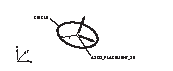
\includegraphics[width=\linewidth]{img/circle_entity.pdf}
	
	\caption{Visualisierung \textit{CIRCLE}}
	\label{fig:circleentity}
\end{figure} 

\paragraph{PLANE}

Beschreibt eine Ebene im Raum. Diese Ebene hat keine räumliche Begrenzung und ist durch einen \textit{AXIS2\_PLACEMENT\_3D} eindeutig definiert. Ähnlich wie beim \textit{CIRCLE} legt der erste Vektor des lokalen Koordinatensystems den Normalenvektor der Ebene fest. Der zweite Vektor beschreibt einen Richtungsvektor der Ebene. Durch den Koordinatenursprung des lokalen Koordinatensystems wird der Ortsvektor der Ebene definiert. 

\begin{figure}[h]
	\centering
	
	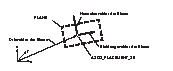
\includegraphics[width=\linewidth]{img/plane_entity.pdf}
	
	
	\caption{Visualisierung \textit{PLANE}}
	
\end{figure} 

\paragraph{CYLINDRICAL\_SURFACE}


Beschreibt analog zur \textit{PLANE} eine zylindrische Ebene im Raum. Diese kann man sich vorstellen als Mantelfläche eines unendlich langen Zylinders. Die Lage des Zylinders wird auch hier durch eine \textit{AXIS2\_PLACEMENT\_3D} definiert und hat als zusätzlichen Parameter eine Zahlenwertangabe zum Radius. In der folgenden Abbildung ist zu erkennen, dass die Achse des Zylinders aus dem ersten Vektor des lokalen Systems gebildet wird und der zweite Vektor parallel zur Deckfläche des Zylinders liegt.

\begin{figure}[h]
	\centering
	
	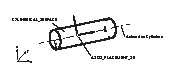
\includegraphics[width=\linewidth]{img/cylinder_entity.pdf}
	
	\caption{Visualisierung \textit{CYLINDRICAL\_SURFACE}}
	
\end{figure}

\paragraph{VERTEX\_POINT}

Definiert einen Punkt des Bauteils im Raum. Dieser wird definiert durch einen \textit{CARTESIAN\_POINT}. Der Unterschied besteht darin, dass es sich bei einem \textit{VERTEX\_POINT} um einen tatsächlichen Punkt des Bauteils (beispielsweise einen Eckpunkt einer Körperkante) handelt und nicht um eine bloße Referenz.   

\paragraph{EDGE\_CURVE}

Beschreibt eine Körperkante. Dabei kann es sich um verschiedene Kantentypen, wie Kreise, Linien oder Splines  handeln. Definiert werden Anfangs- und Endpunkt der \textit{EDGE\_CURVE}. Diese werden als Körperpunkte (\textit{VERTEX}) definiert. Handelt es sich um eine geschlossene Kante, beispielsweise einen Kreis, dann sind Anfangs- und Endvertex identisch. Außerdem weist eine \textit{EDGE\_CURVE} eine Orientierung auf. Diese wird durch einen boolschen Wert (wahr oder falsch) angegeben und definiert so eindeutig Anfangs- bzw. Endpunkt der Körperkante.   

\paragraph{EDGE\_LOOP}

Beschreibt einen Kantenverbund aus mehreren Körperkanten. Dieser Kantenverbund ist geschlossen und enthält als Parameter die Liste der enthaltenen Körperkanten. 

\paragraph{FACE\_OUTER\_BOUND}

Beschreibt die äußere Umrandung einer Körperfläche und wird durch eine \textit{EDGE\_LOOP} beschrieben. Dies kann zum Beispiel ein Polygon aus verschiedenen Linien oder Kurvenstücken sein. Solch eine äußere Umrandung kann aber auch durch einen Kreis definiert sein.

\paragraph{FACE\_BOUND}

Definiert die innere Umrandung einer Körperfläche einer \textit{EDGE\_LOOP}. Dies kann, wie bei einer \textit{FACE\_OUTER\_BOUND}, ein Polygon aus verschiedenen Linien oder Kurvenstücken sein. Solch eine innere Umrandung kann aber auch durch einen Kreis definiert sein.   

\paragraph{ADVANCED\_FACE}

Beschreibt eine tatsächliche Körperfläche des in der STEP-Datei formulierten Bauteils. Definiert ist die Fläche zum einen durch eine Liste an Umrandungen (\textit{BOUND}s) zum anderen durch die Angabe einer PLANE bzw. \textit{CYLINDRICAL\_SURFACE}, in welcher diese Umrandungen liegen. Diese Körperflächen sind in ihrer räumlichen Ausdehnung begrenzt. Die Menge aller \textit{ADVANCED\_FACE}s einer STEP-Datei ergeben zusammengesetzt das beschriebene Modell des Bauteils. 

Abbildung \ref{fig:advancedfaceentity} zeigt den Aufbau einer planaren ADVANCED\_FACE aus einer äußeren Umrandung in Form eines Polygons (EDGE\_LOOP aus mehreren LINE-Entitäten) und einer inneren Umrandung durch einen Kreis.  

\begin{figure}[h]
	\centering
	
	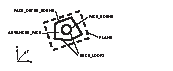
\includegraphics[width=\linewidth]{img/advancedface_entity.pdf}
	
	\caption{Visualisierung planare \textit{ADVANCED\_FACE}}
	\label{fig:advancedfaceentity}
	
\end{figure}

\subsubsection{Bildung einzelner STEP-Entitäten}
\label{sec:string2entity}


Nach der Eingrenzung der zu realisierenden STEP-Entitäten und der Erklärung dieser folgt in diesem Abschnitt die Beschreibung, wie aus einer Zeile der STEP-Datei ein konkretes Java-Objekt gebildet wird. 

Zuerst müssen alle implementierten STEP-Entitäten als Java-Klassen beschrieben werden. Diese dienen als Muster für die verschiedenen Objekte der STEP-Datei. Die oben aufgeführten Klassen sind im Projektordner \textit{"`./src/main/java/com.jandoant/stp\_entities"'} zu finden. Diese enthalten die entsprechend der STEP-Dokumentation aufgeführten Attribute für jede Entität. 

In der Klasse \verb|StpEntityBuilder| im Projektordner \textit{"`./src/main/java/com.jandoant/builder"'} wird dies umgesetzt. Diese Klasse wird im Programmablauf für jede Zeile der STEP-Datei einmal aufgerufen. Übergeben wird ihr die Zeichenkette der jeweiligen Zeile. Aus dieser übergebenen Zeichenkette kann die Klasse nun mit Aufruf der Funktion \verb|extractStpEntity()| ein entsprechendes Objekt der beschriebenen STEP-Entität bilden. 
Dazu wird die beschreibende Zeichenkette in ihre drei Bestandteile (ID, Klassenname, Attributsliste) zerlegt. Über die Kenntnis des Klassennamens kann die Klasse \verb|StpEntityBuilder| entscheiden, welcher Entitätstyp erzeugt werden soll. In einem weiteren Schritt werden die Elemente der Attributsliste extrahiert und ein konkretes Java-Objekt einer STEP-Entität mit all seinen konkreten Attributen kann gebildet werden. Es ist festzustellen, dass es zu diesem Zeitpunkt noch nicht möglich ist, die tatsächlichen Referenzobjekte in der erzeugten Entität festzuhalten. Vorerst kann aus der Zeichenkette nur die jeweilige ID der Referenzobjekte gespeichert werden. Die Zuordnung kann erst erfolgen, wenn alle Zeilen der STEP-Datei in Java-Objekte ausgelesen wurden.

\subsubsection{Abbildung des gesamten STEP-Modells in Java} 

Das Programm ist, wie im vorherigen Abschnitt gezeigt, in der Lage, aus einer einzelnen Zeile der vorliegenden STEP-Datei ein konkretes Java-Objekt zu extrahieren. Nun folgt in diesem Schritt die Decodierung der gesamten Datei. Nach Beendigung dieses Vorgangs ist die komplette geometrische Bauteilstruktur im Programm abgebildet und kann darauffolgend weiter verarbeitet werden.

Der Vorgang dieser Decodierung erfolgt durch die Klasse \verb|StpModelBuilder|, welche sich im Projektordner \textit{"`./src/main/java/com.jandoant/builder"'} befindet. 
Wird diese Klasse im Pro\-gramm\-ab\-lauf instanziiert, so wird ihr der absolute Pfad, unter dem die zu verarbeitende STEP-Datei liegt, übergeben. Mit dieser Information hat die erzeuge Instanz den Zugriff auf alle Zeilen der Datei, welche die Bauteilgeometrie beschreiben.
Mit Aufruf der Funktion \verb|parseFile()| wird die übergebene STEP-Datei verarbeitet. Dabei werden zunächst alle Zeilen der Datei durchlaufen. Jede Zeichenkette, die eine STEP-Entität beschreibt, also mit dem \#-Symbol beginnt und mit einem Semikolon endet, wird in einer Liste dieser Zeichenketten zwischengespeichert. Es ist dabei unerheblich, ob die Zeichenkette durch einen oder mehrere Zeilenumbrüche getrennt ist. Dies hat den Effekt, dass die HEADER-Sektion herausgefiltert wird. Diese hat keine Bedeutung für die grundlegende Funktion des Programms, da in diesem Abschnitt der Datei keine STEP-Entitäten beschrieben werden.

Aus der erzeugten Liste an Zeichenketten, welche dem gewünschten Muster entsprechen, werden im folgenden Bearbeitungsschritt unter Anwendung der in \prettyref{sec:string2entity} dargelegten Methode \verb|extractStpEntity| der Klasse  \verb|StpEntityBuilder| die jeweilig beschriebenen STEP-Entitäten im Java-Code instanziiert und in einer Liste zwischengespeichert. Dabei ist anzumerken, dass ausschließlich die in der Klasse \verb|StpEntityContract| im Projektordner \textit{"`./src/\-main/\-java/\-com.jandoant/\-stp\_entities"'} festgehaltenen STEP-Entitäten decodiert werden. Alle Zeichenketten, die nicht eine solche Entität beschreiben, werden ignoriert. Das führt dazu, dass ausschließlich die geometrischen Informationen des Modells extrahiert werden. Andere Angaben, die in der STEP-Datei festgehalten sein können, werden bei dieser Implementierung nicht berücksichtigt, da sie für die grundlegende Funktion des Programmes unerheblich sind.

Nach dem Durchlaufen aller Zeilen und anschließender Instanziierung der Java-Objekte entsprechend der STEP-Beschreibung liegt zu diesem Punkt eine Liste mit allen vorkommenden geometrischen STEP-Entitäten im Programm vor. Allerdings ist damit den Anforderungen noch nicht entsprochen. Nach der Decodierung der einzelnen Zeichenketten haben die Java-Objekte noch keine Relation zueinander. Wie in \prettyref{sec:string2entity} erläutert, sind die Referenzentitäten, auf die sich eine STEP-Entität bezieht, bisher nur mit ihrer ID erfasst. Eine Zuordnung der Objekte passiert nun aus vorliegender Liste der erzeugten Java-Objekte. 
Dazu wird die Methode \verb|convertFromIds()| aufgerufen, welche in jeder Java-Klasse, die eine STEP-Entität beschreibt, implementiert ist.
Mit Aufruf der Methode durch das betreffende Java-Objekt wird die Entitätsliste durchlaufen. Dabei werden alle Entitäten, deren ID mit einer der IDs, die in diesem Java-Objekt hinterlegt sind, herausgefiltert und dem Java-Objekt zugewiesen. Nachdem dieser Vorgang für alle Objekte der Liste ausgeführt wurde, sind alle Referenzen über tatsächliche Java-Objekte hergestellt. 

Die im Programmablauf aufgerufene Methode \verb|parseFile()| der Klasse \verb|StpModelBuilder| gibt nun in einem finalen Schritt alle \textit{ADVANCED\_FACE}s, die in der STEP-Datei durch Zeichenketten beschrieben wurden, als tatsächliche Java-Objekte an das Programm zurück. Dies geschieht in Form einer Liste. Diese \textit{ADVANCED\_FACE}s  referenzieren wie oben beschrieben alle Objekte, durch welche sie selbst definiert werden. Somit ist die gesamte Bauteilstruktur im Programm abgebildet und kann im weiteren Ablauf des Programms verarbeitet werden.

\subsection{Diskretisierung der Körperflächen}

Die Diskretisierung der Oberflächen wird unter Einführung eines lokalen Koordinatensystems für jede einzelne Körperfläche (\textit{ADVANCED\_FACE}) realisiert.
Ziel ist dabei die Umwandlung der Punkte der Körperflächen, welche durch die STEP-Datei in globalen Koordinaten ausgedrückt sind, in ein lokales Koordinatensystem zu überführen und im Anschluss zu verändern. Dabei werden alle Punkte der jeweiligen Fläche einer Koordinatentransformation unterzogen. So besitzt jeder Punkt neben seiner Beschreibung im Weltkoordinatensystem mit Werten in x-, y- und z-Richtung gleichzeitig auch Definitionen bezüglich eines lokalen Koordinatensystems in u-, v- und w-Richtung. Die folgende \prettyref{fig:basetrafo} verdeutlicht dies. 

\begin{figure}[h]
	\centering
	
	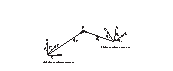
\includegraphics[width=\linewidth]{img/basetrafo.pdf}
	
	\caption{Beschreibung eines Punktes in verschiedenen Koordinatensystemen}
	\label{fig:basetrafo}
	
\end{figure}

Das lokale Koordinatensystem ist spezifisch für jede Körperfläche und ermöglicht eine generalisierte Bearbeitung der diskretisierten Punkte. Jede dreidimensionale Körperfläche wird so in eine zweidimensionale Fläche mit Ausdehnung in u- und v-Richtung überführt. Die w-Koordinate, welche senkrecht zur Fläche zeigt, ist dabei für die Idealgeometrie w = 0. Dieses Verfahren wird als "`UV-Mapping"' bezeichnet. Mit der Anwendung der Deformationsfunktionen ändert sich die Koordinate der Punkte in dieser Richtung. Eine Rücktransformation in das globale Koordinatensystem bildet diese Veränderung an der deformierten Geometrie ab.       

\begin{figure}[h]
	\centering
	
	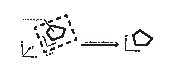
\includegraphics[width=\linewidth]{img/uvwmapping.pdf}
	
	\caption{UV-Mapping einer Körperfläche}
	\label{fig:uvwmapping}
	
\end{figure}
 
\subsubsection{Basistransformation}
\label{sec:basetransform}


Um eine Basistransformation zwischen Welt- und lokalem Koordinatensystem durchführen zu können, ist es notwendig, sowohl die Basiseinheitsvektoren des Weltkoordinatensystems als auch die des lokalen Systems zu kennen. Die Basiseinheitsvektoren des globalen Koordinatensystems sind für alle Punkte des STEP-Modells stets dieselben und werden wie folgt definiert.

\begin{singlespace}
	\begin{equation}
	\begin{aligned}
	\vv{e_{x}}=\begin{pmatrix}
	1 \\ 
	0 \\ 
	0
	\end{pmatrix}  
	&& 
	\vv{e_{y}}=\begin{pmatrix}
	0 \\ 
	1 \\ 
	0
	\end{pmatrix}  
	&& 
	\vv{e_{z}}=\begin{pmatrix}
	0 \\ 
	0 \\ 
	1
	\end{pmatrix} 
	\end{aligned}
	\end{equation}
\end{singlespace}

Die Menge aller Punkte einer Ebene wird in der Geometrie durch die Formel

\begin{equation}\label{eq:plane}
E: \vv{x} = \vv{x_{0}} + r \cdot \vv{x_{R1}} + s \cdot \vv{x_{R2}}  
\end{equation}

eindeutig festgelegt. Dabei steht $\vv{x}$ für einen beliebigen Punkt der Ebene. $\vv{x_{0}}$ beschreibt den Ortsvektor, $\vv{x_{R1}}$ und $\vv{x_{R2}}$  die Richtungsvektoren und $r$ und $s$ sind beliebige Laufparameter, um die Lage des Punktes als Linearkombination der Richtungsvektoren genau zu beschreiben.

Die Position einer \textit{PLANE} wird durch eine \textit{AXIS2\_PLACEMENT\_3D} beschrieben. Daraus lassen sich die Elemente einer Ebenenbeschreibung, wie in \prettyref{eq:plane} dargestellt, auslesen. 
Dabei entspricht der \textit{CARTESIAN\_POINT} der Positionsbeschreibung dem Ortsvektor. Dieser stellt gleichzeitig den Koordinatenursprung des lokalen Koordinatensystems dar. Die erste \textit{DIRECTION} dieser Positionsbeschreibung entspricht dem normalisierten Normalenvektor der Ebene $\vv{n}$, die zweite \textit{DIRECTION} einem normalisierten Richtungsvektor $\vv{x_{R1}}$. Da in der Lagebeschreibung der Ebene nur der Normalenvektor und ein Richtungsvektor dieser Ebene beschrieben sind, wird der fehlende Richtungsvektor durch Bildung des Kreuzproduktes der beiden für ein rechtshändiges System nach \prettyref{eq:crossproduct} erzeugt.

\begin{equation}\label{eq:crossproduct}
\vv{x_{R2}} = \vv{n} \times \vv{x_{R1}}
\end{equation}  

Ebenso, wie bei einer ebenen Fläche, die durch die STEP-Entität \textit{PLANE} beschrieben wird, wird auch bei zylindrischen Flächen des Typs \textit{CYLINDRICAL\_SURFACE} die Ausrichtung des lokalen Koordinatensystems in einem \textit{AXIS2\_PLACEMENT\_3D} festgehalten. Dabei unterscheidet sich allerdings die Bedeutung der \textit{DIRECTION}s der Positionsbeschreibung. Der \textit{CARTESIAN\_POINT} des \textit{AXIS2\_PLACEMENT\_3D} beschreibt dabei die Position des Ortsvektors der Fläche, die erste \textit{DIRECTION} die Richtung der Achse $\vv{n}$ des Zylinders und die zweite \textit{DIRECTION} $\vv{x_{R1}}$ liegt parallel zur radialen Richtung des Zylinders. Mit Hilfe der \prettyref{eq:crossproduct} lässt sich auch hier ein weiterer Vektor bilden, welcher rechtshändig orientiert senkrecht zur Achse und $\vv{x_{R1}}$ ebenfalls in radiale Richtung des Zylinder zeigt. 

Die lokalen Basiseinheitsvektoren \begin{singlespace} $\vv{e_{u}}=\begin{pmatrix}
	e_{u_x} & e_{u_y} & e_{u_z}
	\end{pmatrix}^T $, 
	$\vv{e_{v}}=\begin{pmatrix}
	e_{u_x} & e_{u_y} & e_{u_z}
	\end{pmatrix}^T$ und 
	$\vv{e_{w}}=\begin{pmatrix}
	e_{u_x} & e_{u_y} & e_{u_z}
	\end{pmatrix}^T$ 
\end{singlespace} können somit entsprechend \prettyref{eq:basevectorsuvw}  gebildet werden. Darüber wird definiert, in welche Richtung u-, v- und w-Koordinaten jeweils zeigen. 

\begin{equation}\label{eq:basevectorsuvw}
	\begin{aligned}
	\vv{e_{u}}=\vv{x_{R1}} 
	&& 
	\vv{e_{v}}=\vv{x_{R2}}  
	&& 
	\vv{e_{w}}=\vv{n} 
	\end{aligned}
\end{equation}

Sind die Basiseinheitsvektoren der beiden Koordinatensysteme bekannt, so lassen sich die jeweiligen Basismatrizen  durch spaltenweise Aneinanderreihung der Vektoren bilden. Die Basis des Weltkoordinatensystems ergibt sich damit zur Basismatrix $B_{XYZ}$ nach \prettyref{eq:basematrixxyz}. 

\begin{singlespace}
	\begin{equation}\label{eq:basematrixxyz}
		B_{XYZ} = \begin{pmatrix}
		1 & 0 & 0 \\ 
		0 & 1 & 0 \\ 
		0 & 0 & 1
		\end{pmatrix} 
	\end{equation} 
\end{singlespace}

Die Basis des Weltkoordinatensystems ergibt sich analog zur Basismatrix $B_{UVW}$ nach \prettyref{eq:basematrixuvw}.

\begin{singlespace}
	\begin{equation}\label{eq:basematrixuvw}
	B_{UVW} = \begin{pmatrix}
	e_{u_x} & e_{v_x} & e_{w_x} \\ 
	e_{u_y} & e_{v_y} & e_{w_y} \\ 
	e_{u_z} & e_{v_z} & e_{w_z}
	\end{pmatrix} 
	\end{equation} 
\end{singlespace}

Die Transformationsmatrix, um einen Punkt vom globalen in das lokale Koordinatensystem der Ebene zu transformieren, ergibt sich nach \prettyref{eq:matrixXYZ2UVW}.

\begin{equation}\label{eq:matrixXYZ2UVW}
T_{xyz \rightarrow uvw} = B_{uvw}^{-1} \cdot B_{xyz}  
\end{equation}   

Die Transformationsmatrix, um einen Punkt wieder aus dem lokalen Koordinatensystem der Ebene zurück in das globale System zu überführen, ergibt sich nach \prettyref{eq:matrixUVW2XYZ} aus der Inversen der in \prettyref{eq:matrixXYZ2UVW} berechneten Transformationsmatrix.

\begin{equation}\label{eq:matrixUVW2XYZ}
T_{uvw \rightarrow xyz} = T_{xyz \rightarrow uvw}^{-1} 
\end{equation}   

Hat man einen Punkt $\vv{p_{xyz}}$ in globale Koordinaten gegeben, so berechnet sich seine Position im lokalen Koordinatensystem entsprechend \prettyref{eq:trafoxyz2uvw}. 

\begin{equation}\label{eq:trafoxyz2uvw}
\vv{p_{uvw}}=T_{xyz \rightarrow uvw} \cdot \vv{p_{xyz}}
\end{equation}

Analog dazu berechnet man die Rücktransformation eines Punktes $\vv{p_{uvw}}$ vom lokalen Koordinatensystem in das globale Koordinatensystem nach \prettyref{eq:trafouvw2xyz}.
  
\begin{equation}\label{eq:trafouvw2xyz}
\vv{p_{xyz}}=T_{uvw \rightarrow xyz} \cdot \vv{p_{uvw}}
\end{equation}

Die Berechnung einer speziellen Transformationsmatrix ist in den Klassen \verb|StpPlane|, für planare Ebenen sowie \verb|StpCylindricalFace|, für zylindrische Oberflächen implementiert.  Diese befinden sich im Projektordner \textit{"`./src/main/java/com.jandoant/stp\_entities"'}.\\ 
Die Methode \verb|getXYZtoUVWTransformationMatrix()| ermittelt die Transformationsmatrix für die Umwandlung eines Punktes in lokale Koordinaten. Die Matrix zur Rücktransformation wird über die Methode \verb|getUVWtoXYZTransformationMatrix()| berechnet. 
Die Anwendung dieser Matrizen erfolgt in der Klasse \verb|StpCartesianPoint| im selben Projektordner.\\ 
Die Methode \verb|baseTransform(Matrix transformationMatrix)| nimmt eine Transformationsmatrix entgegen und gibt einen entsprechend der Formeln \ref{eq:trafoxyz2uvw} bzw. \ref{eq:trafouvw2xyz} transformierten Punkt aus. 

\subsubsection{Diskretisierung zylindrischer Flächen}

Zylindrische \textit{ADVANCED\_FACE}s werden in einer STEP-Datei durch eine \textit{CYLINDRICAL\_SURFACE} und zwei\textit{CIRCLE}s definiert. Dabei entspricht die \textit{CYLINDRICAL\_SURFACE}, wie in \prettyref{sec:erklaerungstp} bereits erläutert, der Mantelfläche des Zylinders. Die Begrenzungen des Zylinders ergeben sich aus der Lage der beiden Kreise (STEP-Entität \textit{CIRCLE}), die als \textit{FACE\_\-OUTER\_\-BOUND}s in der STEP-Datei formuliert sind. Der Abstand der beiden Kreise ergibt somit die gesamte Länge der zylindrischen Körperfläche.

Um eine zylindrische \textit{ADVANCED\_FACE} zu diskretisieren, müssen die Positionen der \textit{CYLINDRICAL\_SURFACE} und der \textit{CIRCLE}s, gegeben durch jeweils ein \textit{AXIS2\_PLACEMENT\_3D}, gefunden werden. Im Anschluss werden diese Positionen aus dem globalen in ein lokales Koordinatensystem transformiert. Dies ermöglicht einen generalisierten Diskretisierungsvorgang für Zylinder, unabhängig von ihrer Lage im Raum. Die Transformationsmatrix für eine \textit{CYLINDRICAL\_SURFACE} ergibt sich, wie im vorherigen Abschnitt \ref{sec:basetransform} beschrieben.  

\begin{figure}[h]
	\centering
	
	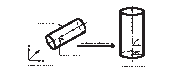
\includegraphics[width=\linewidth]{img/trafozylinder.pdf}
	
	\caption{Koordinatentransformation \textit{CYLINDRICAL\_SURFACE}}
	\label{fig:trafozylinder}
	
\end{figure}

Die Abwicklung der zylindrischen Mantelfläche ergibt ein Rechteck. Dieses entspricht in seiner Breite dem Umfang des Kreisprofils des Zylinders und in der Höhe der Länge des Zylinders. Eine Rechteckfläche ist sehr einfach durch ein gleichmäßiges Punkteraster zu diskretisieren. Dabei ist es notwendig, zuerst die Abwicklung durchzuführen. Über die Transformation der lokalen kartesischen Koordinaten in u-, v- und w-Richtung in lokale zylindrische Koordinaten soll dies umgesetzt werden. Nach erfolgter Transformation in das zylindrische Koordinatensystem kann jeder Punkt auf der Zylinderoberfläche als Punkt auf der abgewickelten Mantelfläche in zylindrischen Koordinaten ausgedrückt werden. \prettyref{fig:discretzylinder} soll den Sachverhalt darstellen. 

\begin{figure}[h]
	\centering
	
	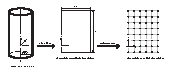
\includegraphics[width=\linewidth]{img/discretzylinder.pdf}
	
	\caption{Abwicklung und Diskretisierung einer zylindrischen Körperfläche}
	\label{fig:discretzylinder}
	
\end{figure}

Die Transformation eines kartesischen Punktes der Zylinderoberfläche kann mit den folgenden Formeln in einen Punkt in zylindrischen Koordinaten umgerechnet werden.
Wenn gilt 
\begin{singlespace}
 \begin{equation}
 	\begin{aligned}
	 	\vv{p_{uvw}} = \begin{pmatrix}
	 	u & v & w
	 	\end{pmatrix}^T \\
	 	\vv{p_{r\varphi w}} = \begin{pmatrix}
	 	\varphi & w & r
	 	\end{pmatrix}^T	 	 	
	 \end{aligned}
 \end{equation}
\end{singlespace}
dann ergeben sich die zylindrischen Koordinaten bei gegebenen kartesischen Koordinaten nach
\begin{equation}	
	\begin{aligned}
		r &= \sqrt{u^2 + v^2} \\
		\varphi &= {\arctan{\frac{v}{u}}}
	\end{aligned}	
\end{equation}
Der Wert in w-Richtung ändert sich dabei nicht.

Analog dazu lässt sich auch die Rücktransformation in kartesische Koordinaten bei gegebenen zylindrischen Koordinaten durchführen. Auch dabei ändert sich die w-Koordinate nicht.
\begin{equation}\label{eq:cyl2uvw}	
	\begin{aligned}
		u &= r \cdot \cos{\varphi}  \\
		v &= r \cdot \sin{\varphi}
	\end{aligned}	
\end{equation}

Um die Diskretisierung einer gegebenen zylindrischen \textit{ADVANCED\_FACE} durchzuführen, ist es also notwendig, diese abgewickelte Rechteckfläche mit einem Punkteraster zu versehen. Der Nutzer kann dabei angeben, in wieviele axiale Ringe und wieviele Zylindersegmente die Fläche zerlegt werden soll. Aufgrund dieser Angaben wird das Punkteraster entsprechend erstellt. Das Programm berechnet aus der gewünschten Anzahl der Ringe die Abstände in w-Richtung, aus der Angabe der Anzahl der Zylindersegmente den Abstand in $\varphi$-Richtung. Beginnend bei der w-Koordinate des Mittelpunkts des ersten \textit{CIRCLE}s und der Winkelkoordinate $\varphi = 0$ wird das Raster bis zur w-Koordinate des zweiten \textit{CIRCLE}s und $\varphi = 2\pi$ in den benötigten Abständen aufgezogen. Jeder erzeugte Punkt des Rasters wird in der Punktewolke der \textit{ADVANCED\_FACE} gespeichert und kann bei Deformation der Fläche verändert werden. 

\subsubsection{Diskretisierung planarer Flächen}
\label{sec:discreteplanar}

Planare \textit{ADVANCED\_FACE}s werden in STEP durch die \textit{PLANE}, auf der sie liegen, und einer bestimmten Anzahl an Umrandungen beschrieben. Die Menge aller Punkte, die zu dieser \textit{ADVANCED\_FACE} gehören, ergibt sich aus der Schnittmenge aller Punkte der \textit{PLANE} und den Punkten innerhalb der positiven Umrandungen (\textit{FACE\_OUTER\_BOUND}s) ohne die Punkte, die innerhalb der negativen Umrandung liegen. 
Dies ist durch folgende Abbildung zu visualisieren.

\begin{figure}[h]
	\centering
	
	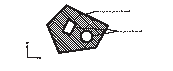
\includegraphics[width=\linewidth]{img/posnegbounds.pdf}
	
	\caption{Planare \textit{ADVANCED\_FACE} mit negativen Umrandungen}
	\label{fig:posnegbounds}
	
\end{figure}

Bei der Diskretisierung planarer Flächen wird unterschieden zwischen kreisförmigen Umrandungen und Umrandungen, die aus einem Polygon bestehen.

Als erstes soll die Diskretisierung von positiven kreisförmigen Umrandungen beschrieben werden. Dazu wird die kreisförmige Fläche in Ringe und Segmente unterteilt. Der Nutzer kann für jede Umrandung die Anzahl dieser angeben und somit die Detaillierung der Diskretisierung steuern. Die Schnittpunkte dieser Elemente sollen als Objekte der Klasse \verb|StpCartesianPoint| in der Punktewolke der Körperfläche gespeichert werden. 

\begin{figure}[h]
	\centering
	
	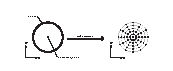
\includegraphics[width=\linewidth]{img/discretcircle.pdf}
	
	\caption{Diskretisierungsmuster Kreis}
	\label{fig:discretecircle}
	
\end{figure}

Wie in \prettyref{sec:erklaerungstp} beschrieben, besteht eine einzelne Umrandung einer \textit{ADVANCED\_FACE} aus einem Kantenverbund (\textit{EDGE\_LOOP}). Bei kreisförmigen Umrandungen wird dieser Kantenverbund genau aus einer Kante des Typs \textit{CIRCLE} gebildet. Diese Entität enthält Informationen zur Position des Kreises (in Form einer \textit{AXIS2\_PLACEMENT\_3D}) und dessen Radius.
Mit dieser Kenntnis kann die Lage des Kreises, bezogen auf das lokale Koordinatensystem, bestimmt werden. Dazu muss auch der Mittelpunkt des Kreises in das lokale Koordinatensystem transformiert werden. Ausgehend vom Radius des zu diskretisierenden Kreises und der Angabe der Anzahl an geforderten Ringen, errechnet das Programm den radialen Abstand der Ringe zueinander. Aus der Anzahl der geforderten Segmente sind in gleicher Weise auch die Öffnungswinkel der Segmente bekannt. Um nun die diskretisierte Punktemenge der Kreisfläche zu erzeugen, wird ein Startpunkt gewählt, welcher auf dem Kreis liegt. Dieser wird um den Mittelpunkt des Kreises und den Öffnungswinkel der Kreissegmente gedreht. Seine neue Position wird in der Punktewolke der betreffenden \textit{ADVANCED\_FACE} gespeichert. Danach wird dieser Vorgang wiederholt, bis die Summe der überstrichenen Öffnungswinkel 360° beträgt. Als Ergebnis dieses Vorgangs entsteht nun ein diskretisierter Ring mit dem Radius des Kreises. Nach Bildung des ersten Ringes wird ein neuer Startpunkt gewählt und von diesem aus analog ein weiterer Ring erzeugt. Dieser Vorgang wird so oft wiederholt, bis die geforderte Anzahl an Ringen hergestellt ist. 

Die Diskretisierung positiver polygonaler Umrandungen geschieht ein wenig anders. Dabei sollen sowohl die Kanten als auch der Innenraum des Polygons entsprechend \prettyref{fig:discretpolygon} in einem vom Nutzer wählbaren Abstand der Punkte  diskretisiert werden. Dazu sollen in einem ersten Schritt alle Kanten des Polygons im vorgegebenen Abstand unterteilt werden. Danach soll ein Punkteraster mit Punkten dieses Abstandes über das Innere des Polygons gelegt werden. Dazu ist es notwendig, alle Eckpunkte, die das Polygon besitzt, zu finden. Das geschieht über den Kantenverbund der (\textit{EDGE\_LOOP}) Umrandung. Dieser ist, anders als bei kreisförmigen Umrandungen, aus mindestens 3 Kanten aufgebaut. Diese Kanten sind vom Typ \textit{LINE}. Aus der einzelnen Kante lassen sich sowohl Anfangs- als auch Endpunkt der \textit{LINE} auslesen. Somit lassen sich die Eckpunkte des Polygons extrahieren. Nachdem die Menge der Eckpunkte des Polygons ermittelt wurde, werden alle diese Punkte in das lokale Koordinatensystem der Ebene unter Anwendung der Transformationsmatrix umgerechnet.
Aus der Kenntnis der Eckpunkte kann nun ein Punkt entlang der Kanten im vorgegebenen Abstand bewegt werden. Nach jedem Einzelschritt wird der Punkt der Punktewolke der \textit{ADVANCED\_FACE} hinzugefügt. 
Um das Innere des Polygons zu diskretisieren, muss zunächst das umgrenzende Rechteck gefunden werden. Innerhalb der Grenzen dieses Rechtecks wird ein Punkteraster im vorgegebenen Abstand erzeugt. Für jeden Punkt wird individuell entschieden, ob er inner- oder außerhalb des Polygons liegt. Liegt ein Punkt dieses Rasters innerhalb des Polygons, dann wird er zur Punktewolke der Körperfläche hinzugefügt.  

\begin{figure}[h]
	\centering
	
	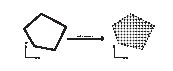
\includegraphics[width=\linewidth]{img/discretpolygon.pdf}
	
	\caption{Diskretisierungsmuster Polygon}
	\label{fig:discretpolygon}
	
\end{figure}

Alle Punkte, die innerhalb einer negativen Umrandung (kreisförmig oder polygonal) liegen, sollen aus der bestehenden Punktewolke der betreffenden \textit{ADVANCED\_FACE} entfernt werden. Dazu wird für jeden bestehenden Punkt geprüft, ob dies der Fall ist. Um allerdings die Kanten negativer Umrandungen in der Punktewolke zu behalten, werden diese entsprechend der Parameter unterteilt und der Punktwolke hinzugefügt.

\subsection{Deformation der Körperflächen}

Die Deformation der einzelnen Punkte einer Körperfläche wird über die Anwendung dreidimensionaler Funktionen realisiert. Die Punkte liegen zu diesem Zeitpunkt des Programmablaufs in lokalen Koordinaten vor. Dabei haben Punkte, die auf einer \textit{PLANE} liegen, Koordinaten in u-, v- und w-Richtung. Bei diesen werden die Werte in w-Richtung durch die jeweilige Deformationsfunktion der Form $w = w_0 + f(u,v)$ verändert. Punkte, welche auf einer \textit{CYLINDRICAL\_SURFACE} liegen, haben hingegen lokale Koordinaten in $\varphi$-, w- und r-Richtung. Die R-Koordinate wird dabei durch eine Deformationsfunktion der Form $r=r_0+f(\varphi, w)$ berechnet. Die Werte $w_0$ bzw. $r_0$ stellen dabei den Wert der jeweiligen Koordinate vor Anwendung der Deformation dar.
Es können für jede Körperfläche unterschiedlich viele Deformationen beaufschlagt werden. Dies führt zu einer Kumulation der Verschiebungen. Damit kann man unterschiedliche Oberflächenabweichungen überlagern.
Die verschiedenen Deformationsfunktionen sind im Quellcode unter dem Projektordner \textit{"`./src/\-main/\-java/\-com.jandoant/deformation"'} zu finden. Jede Klasse in diesem Ordner stellt jeweils eine Deformationsfunktion dar. Diese implementieren alle das Interface \verb|DeformationFunction| im selben Ordner. Das dient dazu, dass alle Deformationsfunktionen der oben beschriebenen Form entsprechen und der Funktionswert stets von zwei Variablen abhängig ist. Zur Anwendung kommt eine Deformationsfunktion durch den Aufruf der Methode \verb|applyDeformationFunction(DeformationFunction df)| der Klasse \verb|StpAdvancedFace| im Ordner \textit{"`./src/\-main/\-java/\-com.jandoant/stp\_entites"'}. Durch die Anwendung der Funktion addieren sich die dritte Koordinate des jeweiligen Punktes und der Funktionswert der Deformationsfunktion an der Stelle des Punktes. So wird die w- bzw. $\varphi$-Koordinate des durch die Deformation verschobenen Punktes gebildet. Im Programm sind ein paar beispielhafte Funktionen definiert. Aufgabe einer Weiterentwicklung des Programms ist Erweiterung und Optimierung dieses Angebotes an Deformationsfunktionen, um Oberflächenabweichungen realistisch abbilden zu können.

Im Folgenden sollen die bereits implementierten Funktionen kurz vorgestellt werden. Dabei werden die Funktionen zur Veränderung planarer Flächen dargestellt. Diese lassen sich aber ebenfalls für zylindrische Flächen anwenden, wenn man u- und v-Koordinate jeweils durch $\varphi$ und w-Koordinate des Zylinders ersetzt. 

\paragraph{Konstanter Faktor} Auf die Fläche wird ein konstantes Offset aufgegeben. Bei ebenen Flächen führt dies zu einer Absenkung oder Anhebung der Fläche in Normalenrichtung der Ebene. Bei Zylindrischen Flächen führt die Anwendung zu einer Erhöhung oder Verringerung des Radius. 
Die Funktion folgt der folgenden Vorschrift. Sie ist implementiert in der Klasse \verb|DeformConstant| und erhält als Parameter den zu verwendenden konstanten Wert. 
\begin{equation}\label{eq:constant}
	w=f(u,v) = \mathrm{c_0}
\end{equation}

\paragraph{Linear in einer Richtung} Wird auf eine ebene Fläche diese Funktion aufgegeben, dann bildet sich eine schiefe Ebene in der angegebenen Richtung. Bei der Verwendung der Funktion auf zylindrische Flächen ergibt nur die Anwendung in axialer Richtung Sinn. So kann bei zylindrischen Flächen eine konische Form hergestellt werden. Die Funktion folgt der folgenden Vorschrift und erhält als Parameter den Anstieg $\mathrm{c_1}$, die Verschiebung $\mathrm{c_0}$ der Punkte senkrecht zur Ebene bzw. Achse und die Richtung der Neigung. 

\begin{equation}	
	\begin{aligned}\label{eq:linear}
		w=f(u,v) = \mathrm{a_1}\cdot u+\mathrm{c_0}&&\mathrm{bzw.}&&w=f(u,v) = \mathrm{a_1}\cdot v+\mathrm{c_0}
	\end{aligned}
\end{equation}

\prettyref{fig:linearufig} und \prettyref{fig:linearvfig} stellen die Funktion grafisch dar. Implementiert ist die Funktion in der Klasse \verb|DeformLinear|.

\begin{figure}[h]
	\centering
	\begin{tikzpicture}
	\begin{axis}[
	grid=both,
	xlabel=$u$, ylabel=$v$, zlabel=$w$ ]
	\addplot3[surf,shader=faceted] {-x};
	\end{axis}
	\end{tikzpicture}
	\caption{Beispiel für lineare Deformation in u-Richtung}
	\label{fig:linearufig}
\end{figure}

\begin{figure}[h]
	\centering
	\begin{tikzpicture}
	\begin{axis}[
	grid=both,
	xlabel=$u$, ylabel=$v$, zlabel=$w$ ]
	\addplot3[surf,shader=faceted] {3*y+4};
	\end{axis}
	\end{tikzpicture}
	\caption{Beispiel für lineare Deformation in v-Richtung}
	\label{fig:linearvfig}
\end{figure}

\paragraph{Linear in zwei Richtungen} Ähnlich wie bei der vorher beschriebenen Funktion erzeugt diese Deformation eine schiefe Ebene. Allerdings ist die erzeugte Fläche in zwei verschiedenen Richtungen geneigt. Sie folgt der folgenden Gleichung. 

\begin{equation}\label{eq:bilinear}
w=f(u,v) = \mathrm{a_1}\cdot u+ \mathrm{b_1}\cdot v+\mathrm{c_0}
\end{equation} 

Diese Funktion ist implementiert in der Klasse \verb|DeformBiLinear|. Sie erhält die Parameter $\mathrm{a_1}$, $\mathrm{b_1}$ und $\mathrm{c_0}$. Diese Funktion wird in \prettyref{fig:bilinearfig} visualisiert.

\begin{figure}[h]
	\centering
	\begin{tikzpicture}
	\begin{axis}[
	grid=both,
		xlabel=$u$, ylabel=$v$, zlabel=$w$ ]
		\addplot3[surf,shader=faceted] {2*x + 3*y+2};
	\end{axis}
	\end{tikzpicture}
	\caption{Beispiel für bilineare Deformation}
	\label{fig:bilinearfig}
\end{figure}

\paragraph{Quadratisch in einer Richtung} Diese Deformationsfunktion funktioniert analog zur linearen Deformation in einer Richtung. Es wird eine gekrümmte Fläche hergestellt. Bei zylindrischen Flächen ergibt sich eine ballige Form, wenn die Funktion in axialer Richtung angewendet wird. Die Funktion wird nach der \prettyref{eq:quadratic} gebildet und ist in der Klasse \verb|DeformQuadratic| implementiert. Übergeben werden die Parameter $\mathrm{a_2}$, $\mathrm{a_1}$ und $\mathrm{c_0}$.  

\begin{equation}\label{eq:quadratic}
	\begin{aligned}
		w=f(u,v) = \mathrm{a_2}\cdot u^2+ \mathrm{a_1}\cdot u+\mathrm{c_0}&&\mathrm{bzw.}&&f(u,v) = \mathrm{a_2}\cdot v^2+ \mathrm{a_1}\cdot v+\mathrm{c_0} 
	\end{aligned}
\end{equation} 

\begin{figure}[h]
	\centering
	\begin{tikzpicture}
	\begin{axis}[
	grid=both,
	xlabel=$u$, ylabel=$v$, zlabel=$w$ ]
	\addplot3[surf,shader=faceted] {0.5*x*x + 1*x -4};
	\end{axis}
	\end{tikzpicture}
	\caption{Beispiel für quadratische Deformation in u-Richtung}
	\label{fig:quadraticu}
\end{figure}

\begin{figure}[h]
	\centering
	\begin{tikzpicture}
	\begin{axis}[
	grid=both,
	xlabel=$u$, ylabel=$v$, zlabel=$w$ ]
	\addplot3[surf,shader=faceted] {-0.5*y*y + 1*y +50};
	\end{axis}
	\end{tikzpicture}
	\caption{Beispiel für quadratische Deformation in v-Richtung}
	\label{fig:quadraticv}
\end{figure} 

\clearpage
\paragraph{Quadratisch in zwei Richtungen} Diese Funktion kann verwendet werden, um eine konvexe bzw. konkave Fläche herzustellen. Sie ergibt sich nach \prettyref{eq:biquadratic} und kann wie in \prettyref{fig:biquadraticfig} visualisiert werden. Die Deformation ist in der Klasse \verb|DeformBiQuadratic| implementiert und erhält als Parameter die Koeffizienten $\mathrm{a_i}$, $\mathrm{b_i}$ und $\mathrm{c_0}$.

\begin{equation}\label{eq:biquadratic}
w=f(u,v) = \mathrm{a_2}\cdot u^2+ \mathrm{a_1}\cdot u+\mathrm{b_2}\cdot v^2+ \mathrm{b_1}\cdot v+\mathrm{c_0}
\end{equation} 


\begin{figure}[h]
	\centering
	\begin{tikzpicture}
	\begin{axis}[
	grid=both,
	xlabel=$u$, ylabel=$v$, zlabel=$w$ ]
	\addplot3[surf,shader=faceted] {-3*x^2+x-2*y^2-4*x+100};
	\end{axis}
	\end{tikzpicture}
	\caption{Beispiel für biquadratische Deformation}
	\label{fig:biquadraticfig}
\end{figure}  


\paragraph{Sinusform in einer Richtung} Um eine wellenförmige Oberfläche zu erzeugen kann diese Deformationsfunktion angewendet werden. Sie folgt der \prettyref{eq:sine} und erhält als Parameter die Werte für Amplitude $\mathrm{a_0}$, Periode $\mathrm{p}$, Phasenverschiebung $\mathrm{\phi_0}$ und dem Offset in w-Richtung $\mathrm{c_0}$ . 

\begin{equation}\label{eq:sine}
w=f(u,v) = \mathrm{a_0} \cdot \sin\left(\frac{p}{2\pi}\cdot x-\frac{2\pi \cdot \phi_0}{p}\right)+\mathrm{c_0}
\end{equation} 

Die Funktion ist in der Klasse \verb|DeformUniDirectionalSine| implementiert und kann durch \prettyref{fig:sineu} oder \prettyref{fig:sinev} werden.

\begin{figure}[h]
	\centering
	\begin{tikzpicture}
	\begin{axis}[
	grid=both,
	xlabel=$u$, ylabel=$v$, zlabel=$w$ ]
	\addplot3[surf,shader=faceted] {0.3*sin(deg(x))};
	\end{axis}
	\end{tikzpicture}
	\caption{Beispiel für sinusförmige Deformation in u-Richtung}
	\label{fig:sineu}
\end{figure} 

\begin{figure}[h]
	\centering
	\begin{tikzpicture}
	\begin{axis}[
	grid=both,
	xlabel=$u$, ylabel=$v$, zlabel=$w$ ]
	\addplot3[surf,shader=faceted] {-1*sin(deg(0.8*y))};
	\end{axis}
	\end{tikzpicture}
	\caption{Beispiel für sinusförmige Deformation in v-Richtung}
	\label{fig:sinev}
\end{figure} 

\clearpage
\subsection{Ausgabe der verformten Geometrie}

Die verformte Geometrie soll als Ergebnis des Programms in einer ASCII-Textdatei ausgegeben werden. Dafür ist es notwendig, dass für alle erzeugten und deformierten Punkte einer Körperfläche diese wieder zurücktransformiert werden. Dies erfolgt entsprechend der \prettyref{eq:trafouvw2xyz}. Für zylindrische \textit{ADVANCED\_FACE}s ist es notwendig, die Rücktransformation in lokale kartesische Koordinaten, wie durch \prettyref{eq:cyl2uvw} beschrieben, vor der Basistransformation durchzuführen. 
Ziel ist die Ausgabe der x-, y- und z-Koordinate jedes Punktes. Dabei entspricht jede Zeile genau einem Punkt. Die Werte sind durch Semikolon getrennt und in der Reihenfolge x, y und z nebeneinander aufgelistet. Die erzeugte Text-Datei kann im Anschluss im Projektordner \textit{"`./src/\-main/\-java/\-com.jandoant/results"'} gefunden und mit jedem Textprogramm ausgelesen werden. Die Rücktransformation und anschließende Ausgabe der Ergebnispunkte einer jeden \textit{ADVANCED\_FACE} ist in der Funktion \verb|print()| der Klasse \verb|StpAdvancedFace| implementiert.

\subsection{Erläuterung eines beispielhaften Programmablaufs}

Die Bedienung des Programms ist zum derzeitigen Stand nur innerhalb der Java-Ent\-wick\-lungs\-um\-geb\-ung \footnote{bspw. IntelliJ IDEA (Community Edition) der Firma Jetbrains,\\ kostenlos herunterladbar unter https://www.jetbrains.com/idea/download} möglich. Da es sich noch um einen frühen Prototypen einer Simulationssoftware für Fertigungsabweichungen handelt, ist noch keine anwenderfreundliche Programmnutzung implementiert. Es soll vorrangig um die Demonstration eines möglichen Programmablaufs gehen. 

Ein beispielhaftes Programm ist in der \verb|MainClass| im Projektordner \textit{"`./src/\-main/\-java/\-com.jandoant"'} hinterlegt. Startet man die \verb|main|-Funktion der Klasse, dann beginnt das Programm mit dem Einlesen der Datei, welche der Instanz der Klasse \verb|StpModelBuilder| übergeben wird. Diese Übergabe, erfolgt in Form einer Zeichenkette, welche der absoluten Adresse der Datei im Ordnersystem des Computers entspricht.
Nachdem die STEP-Datei eingelesen ist, wird diese im zweiten Schritt durch den Aufruf der Methode \verb|parseFile()| der Klasse \verb|StpModelBuilder| decodiert und in Java-Objekten abgebildet. Als Ergebnis dieser Operation gibt diese Methode eine Liste mit Instanzen der Klasse \verb|StpAdvancedFace| zurück, welche alle \textit{ADVANCED\_FACE}s des Bauteils repräsentieren.

Im nächsten Schritt erfolgt die Diskretisierung der Elemente dieser Liste. 
Dazu wird erst eine Unterscheidung vorgenommen, ob es sich um planare oder zylindrische Körperflächen handelt. 
Handelt es sich um Flächen, die sich auf einer Ebene befinden, werden zuerst alle positiven und danach alle negativen Umrandungen (\textit{BOUND}s) diskretisiert und der Punktemenge der jeweiligen \textit{ADVANCED\_FACE} hinzugefügt oder davon abgezogen. Der Nutzer kann über die Angabe der Parameter \verb|distanceOfPoints| (Punktabstand) für polygonale Umrandungen bzw. \verb|numOfRadialSegments| (Anzahl an Kreissegmenten) und \verb|numOfRings| (Anzahl an Ringen) für kreisförmige Umrandungen die Diskretisierungsparameter, wie in \prettyref{sec:discreteplanar} beschrieben, festlegen.
Handelt es sich bei der betrachteten \textit{ADVANCED\_FACE} hingegen um eine zylindrische Körperfläche, so kann der Nutzer die Parameter \verb|numOfRadialSegments|(Anzahl an Zylindersegmenten) und \verb|numOfRings|(Anzahl an Ringen) angeben. 

Nach dem Ablauf dieses Programmteils liegen alle Körperflächen mit ihren diskretisierten Punkten in der Liste der Instanzen der Klasse \verb|StpAdvancedFace| vor. 
Es ist aber zu betonen, dass der Nutzer in diesem beispielhaften Programmablauf die Paramter nur innerhalb des Quelltextes ändern kann. Es erfolgt keine Aufforderung die Parameter einzugeben.
Weiterhin werden aufgrund der Vereinfachung des Programms, alle zylindrischen Flächen des Modells mit den gleichen Parametern diskretisiert. Analog dazu werden auch alle planaren kreisförmigen und alle planaren polygonalen Umrandungen mit den gleichen Parametern, die für ihren Typ festgelegt wurden diskretisiert. Das ist aber nur in diesem Beispielprogramm  auf diese Weise implementiert, es lassen sich mit den verfügbaren Programmbausteinen auch Programmabläufe gestalten, bei denen individuelle Parameter für jede Körperfläche festlegt werden können und somit eine flexible Anpassung an den benötigten Detaillierungsgrad möglich wird.          

Im folgenden Programmschritt werden die Elemente der Punktewolke der \textit{ADVANCED\_FACE}s entsprechend der angewandten Deformationsfunktionen verformt. In diesem Beispielprogramm werden die ersten drei \textit{ADVANCED\_FACE}s des Bauteils mit verschiedenen Deformationsfunktionen beaufschlagt. Über die Funktion \verb|applyDeformationFunction(DeformationFunction df)| der Klasse \verb|StpAdvancedFace| wird eine der möglichen Deformationsfunktionen angewandt.
Werden mehrere Funktionen für eine \textit{ADVANCED\_FACE} benutzt, summiert sich ihre Wirkung. 

Im letzten Schritt des Programms werden die Koordinaten der Elemente aller Punktewolken des Modells in einer Text-Datei ausgegeben. Dabei werden alle Punkte wieder in das Weltkoordinatensystem transformiert und anschließend in die Text-Datei geschrieben. Die erzeugte Datei ist im Ordner {"`./src/\-main/\-java/\-com.jandoant/results"'} zu finden. 

 

 






         




    




           




           


       

        








    













  

\newpage

% -- Bewertung des Lösungsansatzes / der Ergebnisse
\pagestyle{fancy}
\section{Fazit und Ausblick}

Mit den Überlegungen in dieser Arbeit und dem entwickelten Programm wurde eine Grundlage für ein Software-System geschaffen, welches perspektivisch erwartbare Fertigungsabweichungen bei der Herstellung von Bauteilen simulieren kann.

Es wurde untersucht, welche typischen Abweichungen bei der Fertigung von Werkstücken mit bestimmten Verfahren auftreten. Dabei ist festzustellen, dass qualitativ durchaus charakteristische Fehlerbilder für verschiedene Fertigungsprozesse zu erkennen sind. Allerdings lassen die Untersuchungen nur begrenzt qualitative Aussagen bezüglich der Fehler zu. Das erschwert eine Konzeption der Software mit Hinblick auf die Zielstellung, vom angewandten Fertigungsverfahren direkt auf die zu erwartenden Fehler zu schließen. Es ist aber realistisch, die Art der möglichen Fehler einer Oberfläche nach dem Fertigungsverfahren zu klassifizieren und dem Nutzer bei Auswahl der jeweiligen Körperfläche anzubieten. Die konkreten Werte müssen vom Nutzer auf Grundlage der spezifischen Herstellungseinflüsse selbst ermittelt und getroffen werden. Die zu erwartende Wirkliche Oberfläche des Bauteils ist quantitativ nicht generalisiert vorhersagbar. Mit Kenntnis der Arbeitsweise der verwendeten Werkzeugmaschine, der Produktionsumgebung und der Prozessbedingungen sowie dem Material und dem Verschleißzustand des Werkzeugs lassen sich durch Vergleich mit anderen, unter ähnlichen Bedingungen bereits hergestellten Bauteilen, Vorhersagen treffen.
Diese für jeden Fertigungsprozess zu erlangenden Erkenntnisse müssen in die Software einfließen, sodass zu erwartende Fehler kundenspezifisch simuliert werden können. 

Das entwickelte Programm ist zum derzeitigen Stand in der Lage, eine STEP-Datei des zu untersuchenden Bauteils einzulesen und in einzelne Geometrieelemente zu zerlegen. Für jedes einzelne Geometrieelement lassen sich kontinuierliche Deformationsfunktionen anwenden, welche die ideale Formgestalt des Bauteils ändern. Als Ergebnis werden die räumlichen Koordinaten einer Punktewolke der veränderten Geometrie in einer Text-Datei ausgegeben. 

Es ist zu betonen, dass die vorliegende Software als Grundlage für die Umsetzung einer Simulationssoftware für Fertigungsabweichungen eines vorgegebenen Bauteils zu betrachten ist. Es handelt sich keineswegs um ein bereits praktisch verwendbares Programm.   
Zum derzeitigen Stand sind nur Bauteile, die entweder planare  oder zylindrische Flächen als Geometrieelemente aufweisen, verwendbar. Um andere Geometrien, wie beispielsweise Freiformflächen oder gezogene Profile, verwenden zu können, müsste auf Grundlage der bereits umgesetzten STEP-Entitäten eine Ergänzung der Implementierung anderer Körperflächentypen geschehen. 
Das entwickelte Programm bietet die Möglichkeit, eine ideale Geometrie mit gewünschten Verformungen zu beaufschlagen. Allerdings muss der Katalog um weitere möglichen Deformationsfunktionen erweitert werden. Die bisher verfügbaren Funktionen sollen die angedachte Funktionsweise des Programms verdeutlichen, sind aber noch nicht an die eigentlichen Fertigungsfehler angepasst und optimiert. Um eine tatsächliche Simulationsfunktion der Software umzusetzen, müssen solche Funktionen gefunden werden, die eine Anpassung der Parameter durch den Nutzer erlauben und realistische Fehler abbilden können. 

Bei der Weiterentwicklung des Programms gibt es sehr viel Potential. Neben der angesprochenen Erweiterung des Spektrums an Geometrieelementen und möglichen Deformationen ist auch die Benutzerfreundlichkeit ein wichtiger Aspekt. So ist eine Visualisierung der Geometrie unbedingt notwendig, um die Auswahl der zu verändernden Geometrieelemente für den Nutzer intuitiv zu gestalten. Derzeit ist eine Auswahl einer Körperfläche nur über deren ID möglich, dies stellt jedoch eine sehr umständliche und wenig anwenderfreundliche Art der Bedienung dar. Des weiteren muss ein konkreter Programmablauf, ähnlich dem dargestellten beispielhaften Programmablauf, entwickelt werden. Die Bausteine und Herangehensweise, um dies umzusetzen, sind grundsätzlich durch die Programmierung in dieser Arbeit gegeben.    

Durch die Verwendung kontinuierlicher Funktionen können hauptsächlich Gestaltabweichungen nach DIN 4760 \cite{DIN.4760} umgesetzt werden. Es ist aber perspektivisch auch denkbar, Oberflächenunvollkommenheiten nach DIN EN ISO 8785 \cite{DIN.8785} zu simulieren. Mit dem aus der Computergrafik bekannten Verfahren des Displacement Mappings, wie beispielsweise in \cite{Kalos.2008} beschrieben, lassen sich über diskrete, zum Beispiel in Form von Graustufenbildern, gegebene Verformungsfelder auf Körperflächen projizieren. Dabei ist in jedem Pixel des Graustufenbildes ein Helligkeitswert gespeichert, der ein Maß für die Verschiebung des Punktes an der Stelle des Pixels darstellt. So lassen sich auch singuläre Strukturen, wie Kratzer oder Ausbrüche, auf der Körperoberfläche darstellen. 

Der derzeitig vorhandene Prototyp des Programms muss und kann also noch in vielen Aspekten weiterentwickelt werden, um eine aussagekräftige Simulation typischer Fertigungsabweichungen zu erlauben.    

      



          
\newpage

% -- Zusammenfassung und Ausblick
\pagestyle{fancy}
\section{Zusammenfassung und Ausblick}
\newpage

% -- Abbildungsverzeichnis
\pagestyle{fancy}
\listoffigures
\newpage

% -- Selbstständigkeitserklärung
\pagestyle{empty}
Selbststaendigkeitserklärung
\newpage


% -- Literaturverzeichnis
\pagestyle{fancy}
\printbibliography[
	% Literaturverzeichnis im Inhaltsverzeichnis anzeigen 
	heading=bibintoc]

\end{document}
